% Page settings
\documentclass[notitlepage,12pt]{article}
\usepackage{fancyvrb, verbatim, listings}                                  % Various for inserting/hosting code
\usepackage{setspace}                                                      % Space between lines (customisable)
\usepackage[margin=2.54cm]{geometry}                                       % Set margins (standard is 2.54cm)
\usepackage[UKenglish,cleanlook]{isodate}                                  % Set default date and date display
\usepackage{fancyhdr} \pagestyle{fancy}                                    % Line the top of the page
\usepackage[activate={true,nocompatibility},final,tracking=true,kerning=true,spacing=true,factor=1100,stretch=10,shrink=10]{microtype}
\microtypecontext{spacing=nonfrench}                                       % Change font and minor spacings to look nicer
\setlength{\parskip}{0.5\baselineskip}                                     % Set default paragraph behaviour: skip a line
%\setlength{\parindent}{0pt}                                                % Set default paragraph behaviour: no indent
%% Packages to use:
% Tables + figures
\usepackage{graphicx}                                                      % control over the import of graphics
\usepackage[table,dvipsnames]{xcolor}                                      % Define tables (with colour control)
\usepackage{float}                                                         % Control over graphics + tables float
\usepackage[justify]{ragged2e}                                             % control over text alignment
\usepackage{booktabs}                                                      % caption graphics + tables (with name in bold)
\usepackage[labelfont=bf]{caption} 
\usepackage{subcaption}
% caption graphics + tables (with name in bold)
\usepackage{tikz}                                                          % Draw graphs inline, guide: https://sites.google.com/site/kochiuyu/Tikz
\usetikzlibrary{shapes,decorations,arrows,calc,arrows.meta,fit,positioning}
\tikzset{
    -Latex,auto,node distance =1 cm and 1 cm,semithick,
    state/.style ={ellipse, draw, minimum width = 0.7 cm},
    point/.style = {circle, draw, inner sep=0.04cm,fill,node contents={}},
    bidirected/.style={Latex-Latex,dashed},
    el/.style = {inner sep=2pt, align=left, sloped}
}
\usepackage{pgfplots} \pgfplotsset{compat=1.16}                            % Automatic graphing, read https://www.overleaf.com/learn/latex/pgfplots_package for examples
% Maths + numbers
\usepackage{mathtools}                                                     % Various maths functions
\usepackage{amssymb}                                                       % Various maths functions
\usepackage{amsmath}                                                       % Various maths functions
\usepackage{dsfont}                                                        % Various maths functions
\usepackage{centernot}                                                     % center \not usage
\usepackage{siunitx} \sisetup{round-mode=places, round-precision=3}        % Formalise use of units and numbers among text
\DeclareMathOperator{\eps}{\varepsilon}                                    % epsilon short hand shortcut
\DeclareMathOperator{\st}{\text{ s.t. }}                                   % "such that" short hand shortcut
\DeclareMathOperator{\then}{\text{ then }}                                 % "then" in equation shortcut
\DeclareMathOperator{\ifeq}{\text{ if }}                                   % "if" in equation shortcut
\DeclareMathOperator{\oreq}{\text{ or }}                                   % "or" in equation shortcut
\DeclareMathOperator{\andeq}{\text{ and }}                                 % "and" in equation shortcut
\DeclareMathOperator{\all}{,\; \forall}                                    % all (with spacing) in equation shortcut
\DeclareMathOperator{\N}{\mathbb{N}}                                       % N, natural number, shortcut
\DeclareMathOperator{\R}{\mathbb{R}}                                       % R, real number, shortcut
\DeclareMathOperator{\Ll}{\mathcal{L}}                                     % L, Lagrangian, shortcut
\renewcommand{\vec}[1]{\boldsymbol{\mathit{#1}}}                           % vector notation shortcut
\newcommand{\mat}[1]{\boldsymbol{\mathit{#1}}}                             % matrix notation shortcut
\DeclarePairedDelimiter\abs{\lvert}{\rvert}                                % absolute value notation shortcut
\DeclarePairedDelimiter\norm{\lVert}{\rVert}                               % norm notation shortcut
\newcommand{\Prob}[1]{\Pr\left( #1 \right)}                         % SHortcut for probability notation
\newcommand{\Probgiven}[2]{\Pr\left( #1 \, \middle\vert \, #2 \right)} % SHortcut for probability notation, given
\newcommand{\E}[2][]{\mathbb{E}_{#1} \left[ #2 \right]}                    % Expectation (with optional subscript) shortcut
\newcommand{\Egiven}[3][]{\mathbb{E}_{#1} \left[ #2 \, \middle\vert \, #3 \right]} % Expectation given (with optional subscript) shortcut
\newcommand{\Var}[2][]{\text{Var}_{#1} \left( #2 \right)}                  % Variation (with optional subscript) shortcut
\newcommand{\Cov}[1]{\text{Cov} \left( #1 \right)}                         % Covariance (with optional subscript) shortcut
\newcommand{\median}[1]{\text{median} \left( #1 \right)}                   % Median (with optional subscript) shortcut
\newcommand{\indicator}[1]{\mathds{1}\left\{ #1 \right\}}                  % SHortcut for indicator function
\newcommand{\diff}[2][]{\frac{d#1}{d#2}}                                   % SHortcut for differential fraction as a function
\newcommand{\partialdiff}[2][]{\frac{\partial#1}{\partial#2}}              % SHortcut for partial differential fraction as a function
\newcommand{\converge}[1]{\xrightarrow{ #1 \to\infty}}                     % SHortcut for convergence arrow
\renewcommand{\hat}[1]{\widehat{#1}}                                       % Default estimator notation is widehat
\renewcommand{\bar}[1]{\overline{#1}}                                      % Make over bar look nicer
\renewcommand{\tilde}[1]{\widetilde{#1}}                                   % Make over tilde look better
% Citations
\usepackage[longnamesfirst]{natbib}                                        % Citation package, see https://en.wikibooks.org/wiki/LaTeX/Bibliography_Management#Natbib
\usepackage[backref=page]{hyperref}                                        % Allow for links across the text, with colour options
\hypersetup{colorlinks=true, linkcolor=blue, citecolor=blue, filecolor=magenta, urlcolor=blue}
\def\equationautorefname~#1\null{Equation~(#1)\null}                       % Fix autoref for equations
% IMPORTANT: follow style guide here https://github.com/Wookai/paper-tips-and-tricks


%%%%%%%%%%%%%%%%%%%%%%%%%%%%%%%%%%%%%%%%
%% Title page
% Author
\author{Senan Hogan-Hennessy\thanks{
    Economics Department, Cornell University.}
}
% Title
\title{Changes in Faculty Composition and Stagnating State Support for Higher Education
    }
\date{\today\thanks{
    I thank Professor Evan Riehl for guidance on this project, Michael Lovenheim, Ronald Ehrenberg, Douglas Miller, Francine Blau, and Ryan Dycus for various comments on the project's direction, as well as seminar participants at Cornell University (Autumn 2022) for helpful discussion.
    This project's Github repository, with materials and (publicly available) data for replication, is available at 
    \url{https://github.com/shoganhennessy/state-faculty-composition}.
    Any comments or suggestions may be sent to me at \href{mailto:seh325@cornell.edu}{\nolinkurl{seh325@cornell.edu}}, or raised as an issue on the Github project.
    }
}
\rhead{\today}
\lhead{Faculty Composition and State Support for Higher Education}
% Begin
\begin{document}
\clearpage
\maketitle
\thispagestyle{empty}
% Abstract
\begin{abstract}
    \noindent
State support for higher education has stagnated on a per-student level, while public universities have reduced their employment of tenure-track or tenured professors, and increased their employment of contingent lecturers (per student).
This analysis relates these changes in the faculty composition at public universities to the fall in per-student university revenues from state appropriations.
A shift-share instrumental variables approach addresses endogeneity in decisions for state appropriations to higher education, by exploiting the yearly change in state support with an institution's reliance on that support.
A decrease in state funding of 10\%, via a shock to state appropriations, decreases the number of assistant professors per student at a public university by 1.4\% and full professors by 1.2\%, yet increases the number of lecturers per student by 4.4\%.
Local project estimates show that these effects linger for up to three years after the initial shock.
Analysis of all the professors hired at Illinois public universities 2011-2021 shows that incumbent professors are not affected by the changes in state support, implying that these changes in faculty composition arose by reduced hiring of tenure-track and tenured professors at public universities.
These results exhibit the long-term effects of stagnating state support for higher education, and raises questions about the direction that public education heads as these financial headwinds show no sign of dissipating.

\vspace{0.75cm}
\noindent\textbf{Keywords:}
State and Local Budget and Expenditures,
Higher Education,
Public Sector Labor Markets

\vspace{0.5cm}
\noindent\textbf{JEL Codes:} H72, I23, J45
\end{abstract}

%%%%%%%%%%%%%%%%%%%%%%%%%%%%%%%%%%%%%%%%%
%% Starting the paper
\newpage
\setcounter{page}{1}
\doublespacing
% Introduction section
\noindent
Public universities educate the majority of higher education students in the US, yet have experienced a secular decline in state funding (per student) the last three decades.
This decline has been shown to lead to worse education and later-life outcomes for students \citep{NBERw23736,NBERw27885}, yet it is not clear what mechanisms drive these effects, or how public universities are affected as institutions.
I show that four-year, degree-granting public universities have experienced falling state funding per student, and this affected their composition of faculty.
Falls in public university revenues from the state, instrumented by state-level finance shocks, lead to a fall in the number of tenure-track or tenured professors per student within a university, an increase in the number of lecturers, and overall fall in the number of faculty per student.
US private universities were not exposed to such financial constraints during this same time period, and do not exhibit the substitution away from tenure-track and tenured professors, so that the stagnating state support for public universities has implications for the wider structure of higher education instruction and research in the US.

US universities are widely considered the highest performing in the world, yet there are consequential differences between its universities that operate in the private sector and those established by state governments.
Public universities are subject to numerous state-level administrative laws, and rely on their state governments for funding: an average public university received around \$11,600 per enrolled student in 1990, yet only \$8,300 per enrolled student in 2021.
This fall is driven by stagnating funding provided by state governments, while enrolment among public universities rose by 46\% over the same time period.
At the same time, the number of professors per student at public universities stayed relatively stable at 0.045, yet fell from around 0.04 to around 0.35 professors per student at public universities, driven by a fall of over 20\% in the ratio of associate and full professors per student at public universities.

I use a variant of the \cite{NBERw23736,NBERw27885} shift-share instrument for state funding from shocks to appropriations for the entire state to identify the effect on the faculty composition.
State appropriations for public universities are plausibly endogenous to many outcomes: state governments decide on yearly budgets for their higher education sector, and this process can be influenced by local financial conditions, or even public perceptions of the state's higher education system.
The shift-share instrument interacts reliance on state funding in a base period with the yearly total appropriations per student in the entire state, to exploit both changes in support for higher education and how much each university relies on that support.

Findings show that negative changes in state funding affects faculty composition at public universities, away from tenured and tenure-track professors towards non-tenure track lecturer positions.
A reduction of 10\% in state funding, via a shock to state appropriations, leads to a fall in 1.4\% in the number of assistant professors per student within a university, 1.2\% for full (tenured) professors, and an increase in 4.4\% the number of lecturers per student.
Local projection methods show that these effects linger for a small number of years after the initial revenue shock.
Over this time period, state funding fell by around 35\%, while the count of professors per student fell by 9\%, so that these results show that falls in state funding explain around a third of the observed shift away from tenure-track and tenure professors towards contingent faculty.

Additionally, I use individual level data on professors at Illinois public universities over 2010-2021 to investigate whether the shocks to state funding affected incumbent professors at public universities.
Incumbent professors were not meaningfully affected, in terms of total salary, promotion rate, or rate of leaving the Illinois public university system, yet lecturers' first year salary decreased by 3.8\% in response to a fall in state funding of 10\%.
These findings imply that changes in faculty composition came about by changes in the composition of hiring new professors at the university level.

\cite{NBERw23736} first study the effect of (changes in) public universities' finances on student outcomes by isolating changes in public universities' expenditures on student instruction, addressing endogeneity of expenditures decisions by instrumenting expenditures with state appropriation shocks and limits on tuition price.
\cite{NBERw23736} find that increases in public university spending (via appropriation shocks) increases enrolment and degree completion among students, but corresponding changes in attendance price (via limits on tuition price) do not have an effect.\footnote{
    \cite{miller2022making} further analyse the effects of falls in university revenues, by finding that reductions in public universities tuition prices (suggestively motivated by falling state funding) leads to reductions in provided financial aid.
}
\cite{chakrabarti2018effect,NBERw27885} use the same instrument for public university revenues at the state level, combined with rich information on students' individual-level outcomes, to show that increases in state appropriations lead to degree lower completion time and later-life student debt.
\cite{bound2019public} use another variant of the same approach to show that state-level higher education spending cuts induced public universities to shift toward tuition as their primary source of revenue, and shift institutional resources towards students who pay higher tuition rates.
In a similar vein, \cite{bound2007cohort} document variation in per student state funding for higher education resulting from yearly changes in a state's student-age population; they find that lower per student funding lead to lower higher education completion rate among students.

Faculty are a core component of this country's educational and research-innovation university system, yet their composition within universities, and its relationship with higher education finances has so far not been studied.
\cite{brown2014endowment} presents the closest example by studying how university endowments react to negative financial shocks, exhibiting an association between negative endowment shocks and a fall in tenure-system faculty employed at private universities.
\cite{abe2015implications} present a model for decision-making by university administrators, and posit that a large component of variation in faculty salaries arises from university politics, and not only economic factors such as outside options.
\cite{johnson2009jep,NBERc13879} both empirically document allocation of faculty between research and instruction, and \cite{hemelt2021math} document differences in instructional cost (per student) between departments, primarily thanks to department differences in class size and faculty salaries.
\cite{turner2014impact} document how universities reacted to the Great Recession of 2008, a severe financial shock to state finances and support for higher education.

The number of professors, both in absolute terms and relative to number of students, may be particularly important for quality of instruction and thus educational outcomes.
\cite{angrist1999using} first causally show that reducing class size (via religious ruling) induces an increase in test scores for school-age children, yet the magnitude of this effect is not as clear in the higher education setting.
\cite{bandiera2010heterogeneous} use a fixed effect model, combined with multiple individual observations in a long panel, to find that UK university students perform worse academically in particularly large classes, and the difference is largest for students at the top of the academic distribution.
For the composition of faculty teaching university classes, \cite{bettinger2010does,figlio2015tenure} find US students have better enrolment and learning outcomes from courses taught by contingent or adjunct (i.e. not tenured or on tenure-track) professors (relative to tenured or tenure-track).
\cite{ehrenberg2005tenured} observe a negative association between utilisation of non-tenured instructors and student graduation rates.
My approach focuses on count of professors per student at universities, so does not directly observe individual class-sizes, yet presents considers this a possible mechanism through which stagnating state support for higher education negatively affects student outcomes \citep{NBERw23736,NBERw27885}.

% Data section
%%%%%%%%%%%%%%%%%%%%%%%%%%%%%%%%%%%%%%%%%
%% Data section
\section{Data and Institutional Context}
\label{sec:data}

\subsection{Data Description}
The data used in this analysis come from two primary sources: \citet[IPEDS]{ipeds} regarding institutional information on finances and enrolment, and \citet[IBHED]{ibhed} for data on every professor in the Illinois public university system.

IPEDS is a survey of higher educational institutions in the US, and legally requires institutions to participate in order to receive Federal Title IV student aid.\footnote{
    This statement means that IPEDS does not necessarily cover the universe of US higher education institutions, yet in practice every public university and not for-profit four-year institution is represented.
}
Data are consistent between the years 1990 and 2021,\footnote{
    The years 1987-1989 are represented in these data in an incompletion fashion, so I focus on the years 1990 onwards.
    Year refers to the calendar year of the spring term --- i.e. 1987 refers to the academic year that ran August 1986 to July 1987.
}
and provide information on the total revenues a university received from every source (including state governments), enrolment number, plus faculty count and total expenditures on salaries.\footnote{
    I combine the Urban Institute's 2018 compilation of IPEDS data for the years 1990-2017, and manually combine with raw NCES data regarding the year 2018-2021 for all relevant variables.
    Figures for enrolment, faculty counts and salaries come from the raw NCES version of IPEDS for all years to address inconsistencies in the Urban Institute's data formulation for these variables.
}
I restrict analysis to public, four-year, degree-granting institutions, as these institutions adhere to a standardised concept of faculty profile, where tenure and title of appointment (lecturer, assistant professor, etc.) are relatively standardised.
For-profit institutions employ and enrol a negligible share of professors and students respectively, while students at two-year institutions by majority intend to eventually enrol at a four-year institution \citep{mountjoy2022},\footnote{
    Furthermore, \cite{mountjoy2022} documents the effects of expanding two-year higher education access in the US separately for students who would have and those who would not have otherwise have attended college.
    The high rate of eventual enrolment at four-year institutions among two-year students explains the negative impact of increased access to two-year institutions on students who are diverted away from four-year institutions.
}
so that these institutions are not considered.

IPEDS reports the count of professors employed by position, as well as total salary expenditures by position.
This gives a resulting panel data-set, where each row represents a university-year, and includes columns for university finances, plus total count and average salary\footnote{
    Real salary is computed by scaling nominal salary to 2021 dollars by the CPI-U.
} for professors by position (lecturer, assistant, tenured, total).
\autoref{tab:ipeds-summary} presents summary statistics for relevant variables in these data.

\begin{table}[h!]
    \singlespacing
    \centering
    \caption{IPEDS Summary Statistics, Public Universities Panel 1987--2021}
    \makebox[\textwidth][c]{
\begin{tabular}{@{\extracolsep{5pt}}lcccc} 
\\[-1.8ex]\hline 
\hline \\[-1.8ex] 
Statistic & \multicolumn{1}{c}{Mean} & \multicolumn{1}{c}{St. Dev.} & \multicolumn{1}{c}{Median} & \multicolumn{1}{c}{N} \\ 
\hline \\[-1.8ex] 
Enrollment, full-time equivalent & 11,511 & 10,821 & 7,723 & 18,504 \\ 
State appropriations (millions 2021 USD) & 99 & 125 & 52 & 18,504 \\ 
Total revenues (millions 2021 USD) & 425 & 793 & 158 & 18,504 \\ 
Lecturers count & 60 & 74 & 34 & 17,329 \\ 
Assistant professors count & 113 & 102 & 84 & 17,826 \\ 
Full professors count & 261 & 284 & 162 & 17,929 \\ 
All professors count & 429 & 437 & 284 & 18,504 \\ 
Lecturers mean salary (2021 USD) & 58,212 & 13,244 & 56,215 & 16,686 \\ 
Assistant mean salary (2021 USD) & 74,319 & 13,849 & 72,191 & 17,750 \\ 
Full mean salary (2021 USD) & 99,675 & 23,590 & 95,229 & 17,837 \\ 
All mean salary (2021 USD) & 81,570 & 25,055 & 80,582 & 17,759 \\ 
\hline \\[-1.8ex] 
\end{tabular} 
}
    \label{tab:ipeds-summary}
\end{table}

IPEDS provides information at the university level, yet lacks information on the distribution of salaries and professor count within a university.\footnote{
    IPEDS provides total paid to salary and total faculty employed per university-year, so that I can investigate average professor salary per university-year with IPEDS data.
    Unfortunately, this measure of professors' salaries is particularly crude in measuring on professors' salaries and other individual-outcomes; summary statistics on IPEDS data do not agree with trends in average professor salary over the sample time period \citep{aau2021survey}.
    Similarly, IPEDS reports of the average salary paid to professors at private institutions also disagree with other sources, so are not considered in this analysis.
}
To investigate the distribution, I integrate individual-level data for every public university professor in the state of Illinois between the years 2010-2021.
IBHED hosts the information;
Public Act 96-0266 (effective 1 January 2010) requires that each university report base salary and benefits all administrators, faculty members, and instructors employed by the college or university.\footnote{
    The universities included are all campuses of the nine Illinois public universities: Chicago State University, Eastern Illinois University, Governors State University, Illinois State University, Northeastern Illinois University, Northern Illinois University, Southern Illinois University  (all five campuses), University of Illinois (all four campuses), Western Illinois University.
}
This publicly available data provides the basis to build a panel of Illinois public university professors 2010-2021; I define a professor as an individual by their first plus last name and university pairing, and link this database to IPEDS regarding finances for their employing institution.

The analysis sample represents 16,932 professors in the year 2010 and 15,352 in the year 2021, with summary statistics presented in \autoref{tab:illinois-summary}.
Additionally, further analysis using the first year of a professor's employment focuses on the subset of professors with observed year of hiring between the years 2011 and 2021, representing 1,778 professors in 2011, and 9,099 in 2021.\footnote{
    Summary statistics for this group, which over-represents lecturers compared to assistant and full professors, can be seen in \autoref{tab:illinois-summary-rolling}.
    The reasons for considering the sub-sample with identified year of hire in the range 2011-2021 are explained in \autoref{sec:iv-model-indiv}.
}

\begin{table}[h!]
    \singlespacing
    \centering
    \caption{IBHED Summary Statistics, Professor Panel 2010--2021.}
    \makebox[\textwidth][c]{
\begin{tabular}{@{\extracolsep{5pt}}lcccc} 
\\[-1.8ex]\hline 
\hline \\[-1.8ex] 
Statistic & \multicolumn{1}{c}{Mean} & \multicolumn{1}{c}{St. Dev.} & \multicolumn{1}{c}{Median} & \multicolumn{1}{c}{N} \\ 
\hline \\[-1.8ex] 
Lecturer, percent & 39 & 49 & 0 & 60,926 \\ 
Assistant professor, percent & 33 & 47 & 0 & 60,926 \\ 
Full professor, percent & 12 & 32 & 0 & 60,926 \\ 
Administrator professor, percent & 17 & 37 & 0 & 60,926 \\ 
Lecturer salary (2021 USD) & 27,280 & 25,579 & 17,738 & 23,618 \\ 
Assistant salary (2021 USD) & 79,352 & 37,038 & 75,339 & 19,865 \\ 
Full salary (2021 USD) & 108,411 & 58,988 & 97,978 & 7,228 \\ 
Administrator salary (2021 USD) & 110,020 & 62,547 & 98,258 & 10,215 \\ 
All salary (2021 USD) & 67,755 & 54,259 & 64,750 & 60,926 \\ 
Lecturer benefits (2021 USD) & 1,944 & 7,190 & 0 & 23,618 \\ 
Assistant benefits (2021 USD) & 2,886 & 7,228 & 0 & 19,865 \\ 
Full benefits (2021 USD) & 5,937 & 13,734 & 0 & 7,228 \\ 
Administrator benefits (2021 USD) & 3,129 & 19,465 & 0 & 10,215 \\ 
All benefits (2021 USD) & 2,924 & 11,155 & 0 & 60,926 \\ 
\hline \\[-1.8ex] 
\end{tabular} 
}
    \label{tab:illinois-summary}
\end{table}

\subsection{Trends in Finances, Enrolment, and Faculty Composition}
\label{sec:trends}
A state government plans an annual budget a couple of years ahead of the fiscal year, and the legislature chooses to approve or reject a budget request put forth by the governor's office.\footnote{
    \cite{NBERw23736} present a full discussion of the decision-making process for state appropriations, drawing on administrative records originally analysed by \cite{parmley2009state}.
}
US state governments, by majority, are legally obligated to run a balanced-budget, so that yearly variation in tax revenues (caused by changing economic conditions or otherwise) necessarily affect state expenditures.
This process leads to yearly variation in state appropriations not seen in other revenues sources (such as federal government appropriations), since US states differ in their support for higher education, and are subject to fiscal constraints.
State appropriations to higher education are a particularly attractive area of state spending to absorb such shocks to state finances \citep{delaney2011state}.\footnote{
    \cite{delaney2011state} fully describes the financial environment of state expenditures, and what makes spending on higher education an attractive area for state governments to expand funding during years of higher tax revenues, and retract funding in leaner years.
    An analysis of state expenditures for the years 1980-2004 (overlapping with the sample for this analysis) provides solid evidence for these trends.
}
Additionally, there is yearly variation in the number of higher education students in each state \citep{turner2014impact}, so that per-student state appropriations vary on multiple dimensions.

\autoref{fig:funding} exhibits the trends for the mean public university for the years 1990-2021.
We see a rise in total revenues received by public universities (from all sources), and a notable increase in mean tuition revenues from \$48 million per year-university to \$150 million per year-university.
At the same time, total state appropriations stagnated at around \$100 million per year-university for 1990-2008, falling around 2008 and have not recovered ever since.
While public universities experienced a stagnation in state support, private universities were not exposed to the same constraints, receiving \$37,000 per student in 1990 and \$49,000 in 2021, experiencing no corresponding decline in any specific component.

\begin{figure}[h!]
    \centering
    \singlespacing
    \caption{Mean Total Revenues among Public Universities, by Year.}
    \begin{subfigure}[b]{0.495\textwidth}
        \centering
        \caption{Total, millions \$ 2021 CPI-U.}
        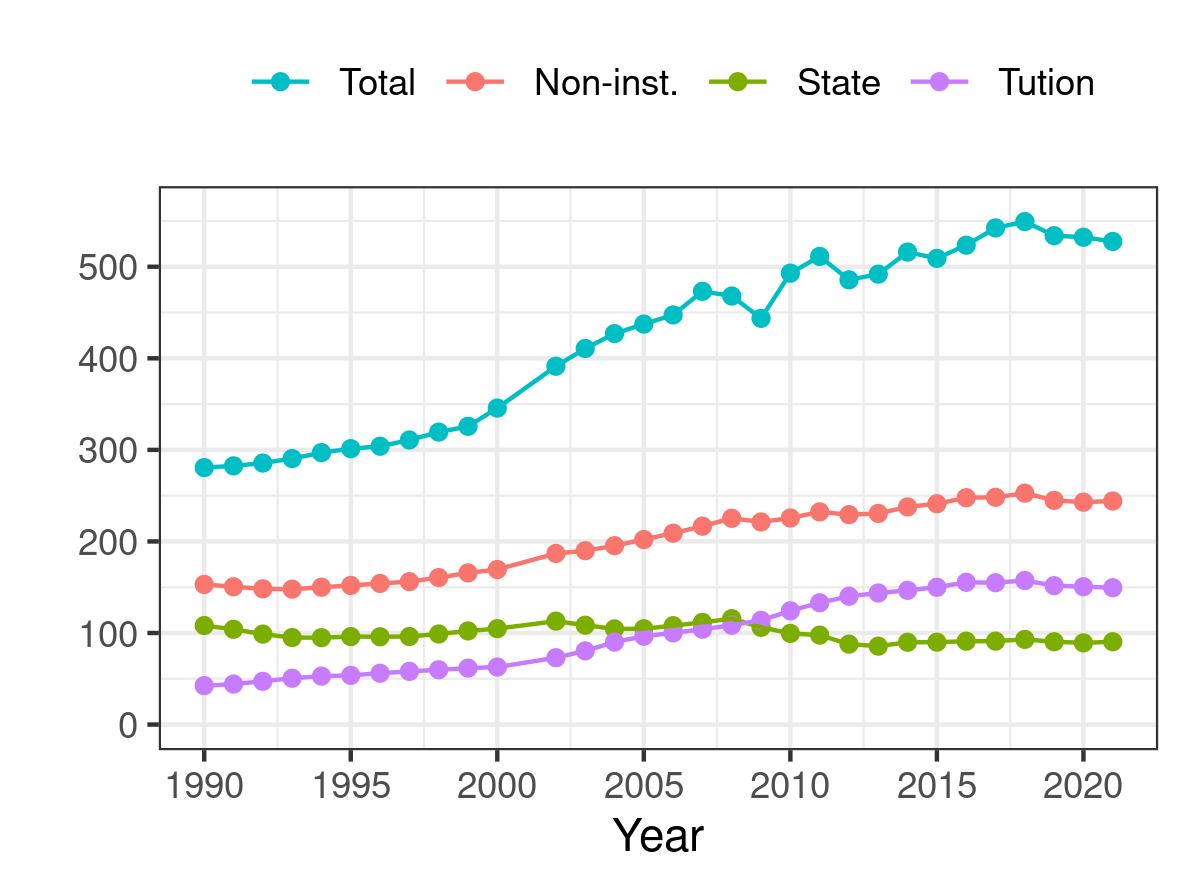
\includegraphics[width=\textwidth]{figures/mean-funding-total.png}
        \label{fig:mean-funding-total}
    \end{subfigure}
    \begin{subfigure}[b]{0.495\textwidth}
        \centering
        \caption{Per Enrolled Student, \$ 2021 CPI-U.}
        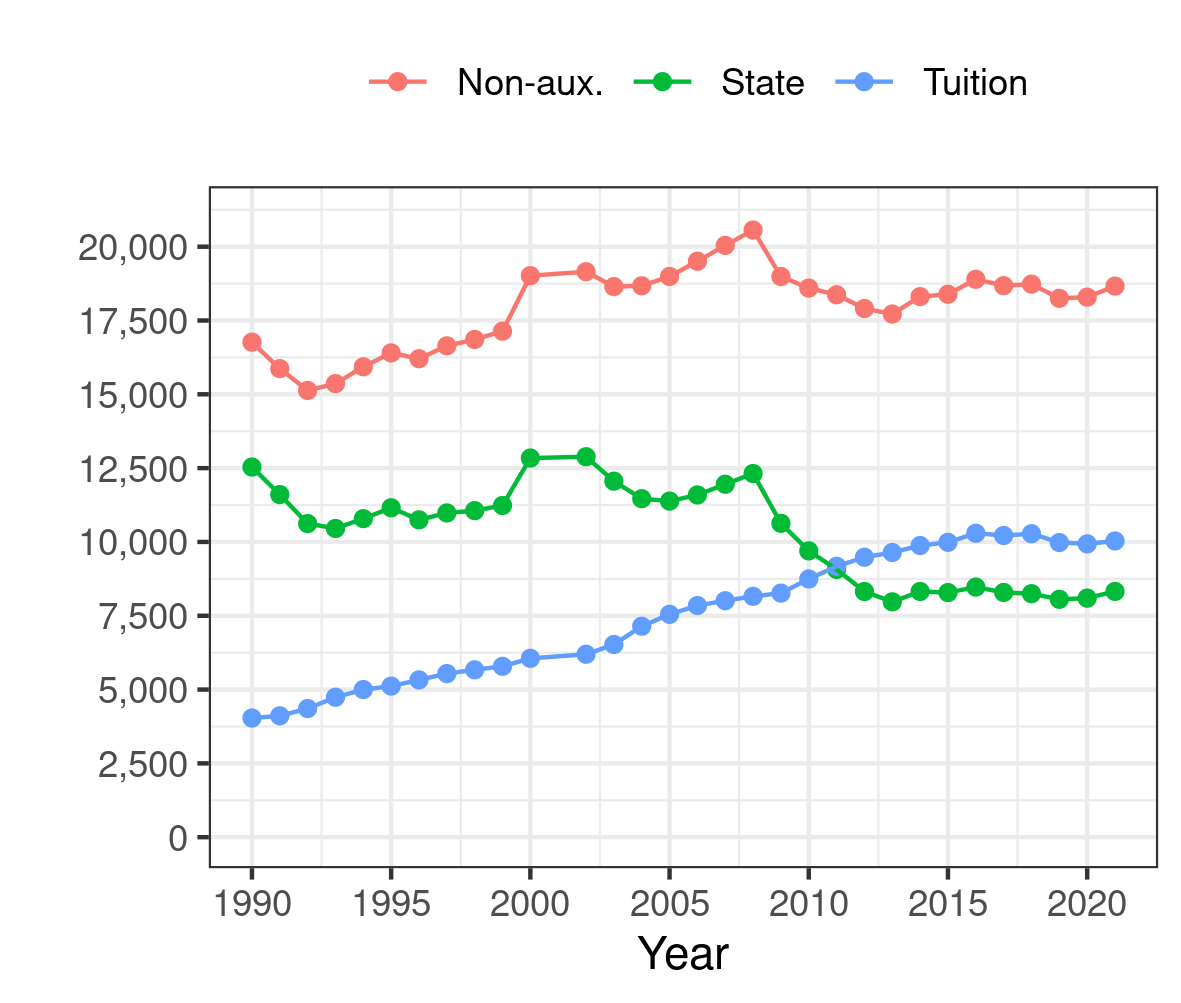
\includegraphics[width=\textwidth]{figures/mean-funding-fte.png}
        \label{fig:mean-funding-fte}
    \end{subfigure}
    \label{fig:funding}
\end{figure}

\begin{figure}[h!]
    \centering
    \singlespacing
    \caption{Total Student enrolment, by University Sector, and Year.}
    \begin{subfigure}[b]{0.495\textwidth}
        \centering
        \caption{Total.}
        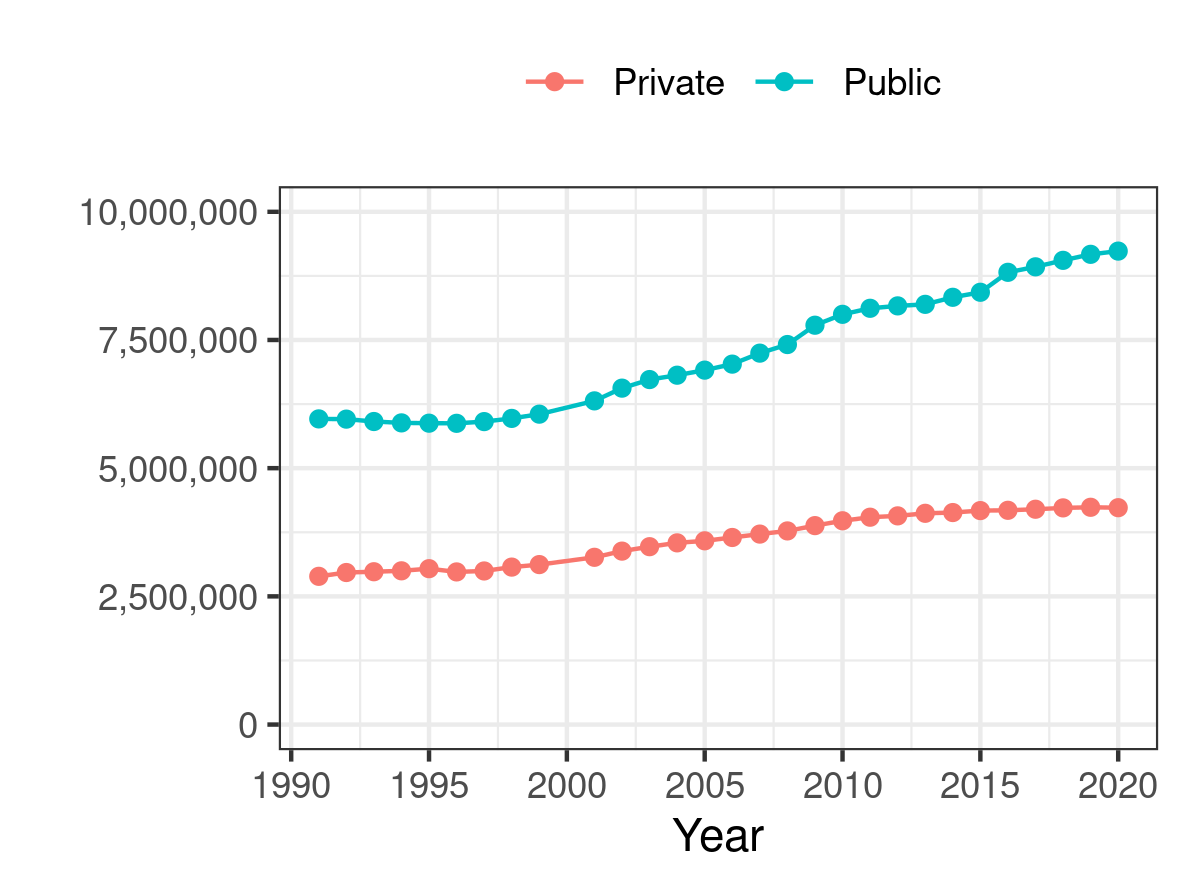
\includegraphics[width=\textwidth]{figures/enrollment-total.png}
        \label{fig:enrollment-total}
    \end{subfigure}
    \begin{subfigure}[b]{0.495\textwidth}
        \centering
        \caption{Mean, University Level.}
        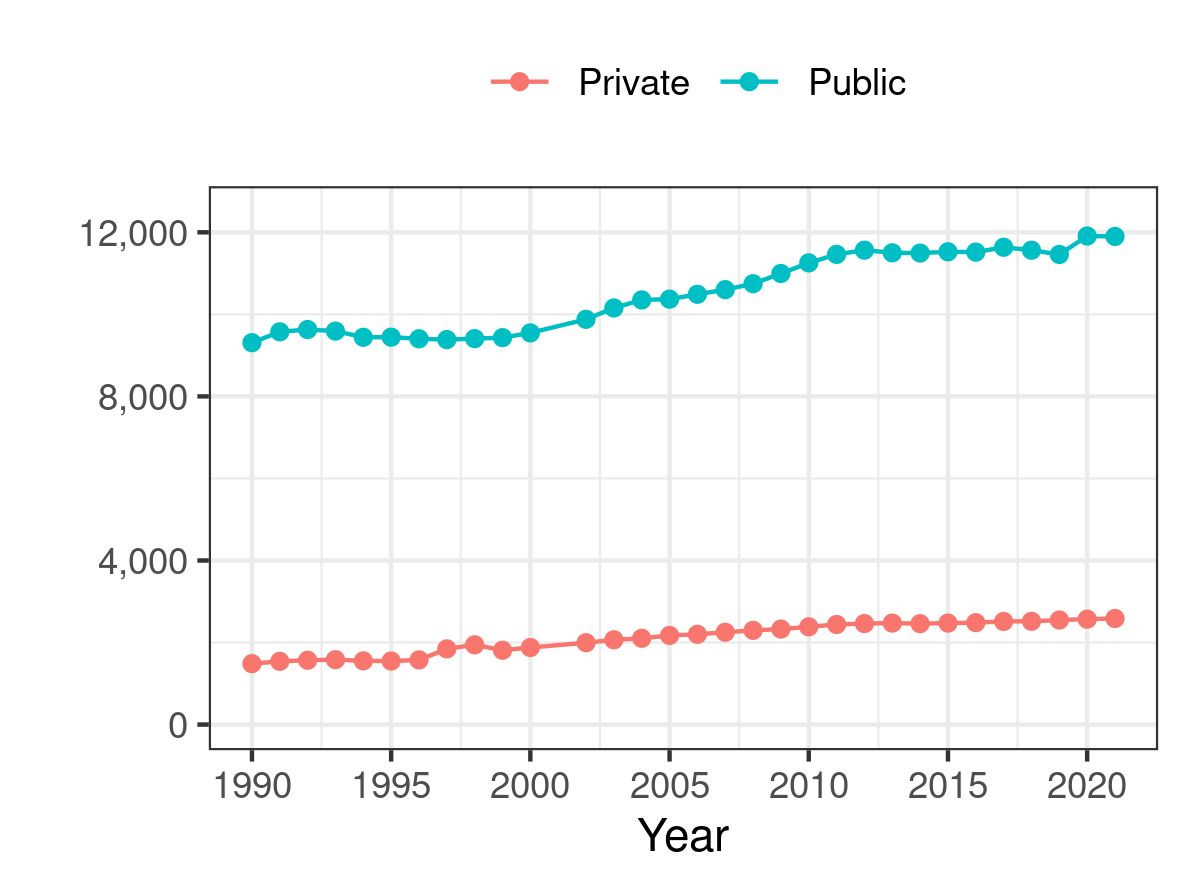
\includegraphics[width=\textwidth]{figures/enrollment-mean.png}
        \label{fig:enrollment-mean}
    \end{subfigure}
    \label{fig:enrolment}
\end{figure}

At the same time, student enrolment at public universities rose precipitously.
6.2 million students were enrolled in public universities in 1990, and this number rose by 47\% to 9.1 million, with most of the increase occurring over the years 2000-2021.
\autoref{fig:enrolment} shows that total enrolment at private universities has also risen over the same time period, but not as drastic in either relative or absolute terms; the mean private university grew from 9,800 students in 1990 to 11,800 in 2021.
This means that revenues per student have stagnated across all measures (seen in \autoref{fig:mean-funding-fte}), and particularly fallen from a mean of \$11,000 per student in 1990 to less than \$8,000 per student in 2021.

\begin{figure}[h!]
    \centering
    \singlespacing
    \caption{Student Enrollment per Professor, by University Sector, Professor Appointment, and Year.}
    \begin{subfigure}[b]{0.495\textwidth}
        \centering
        \caption{Lecturer}
        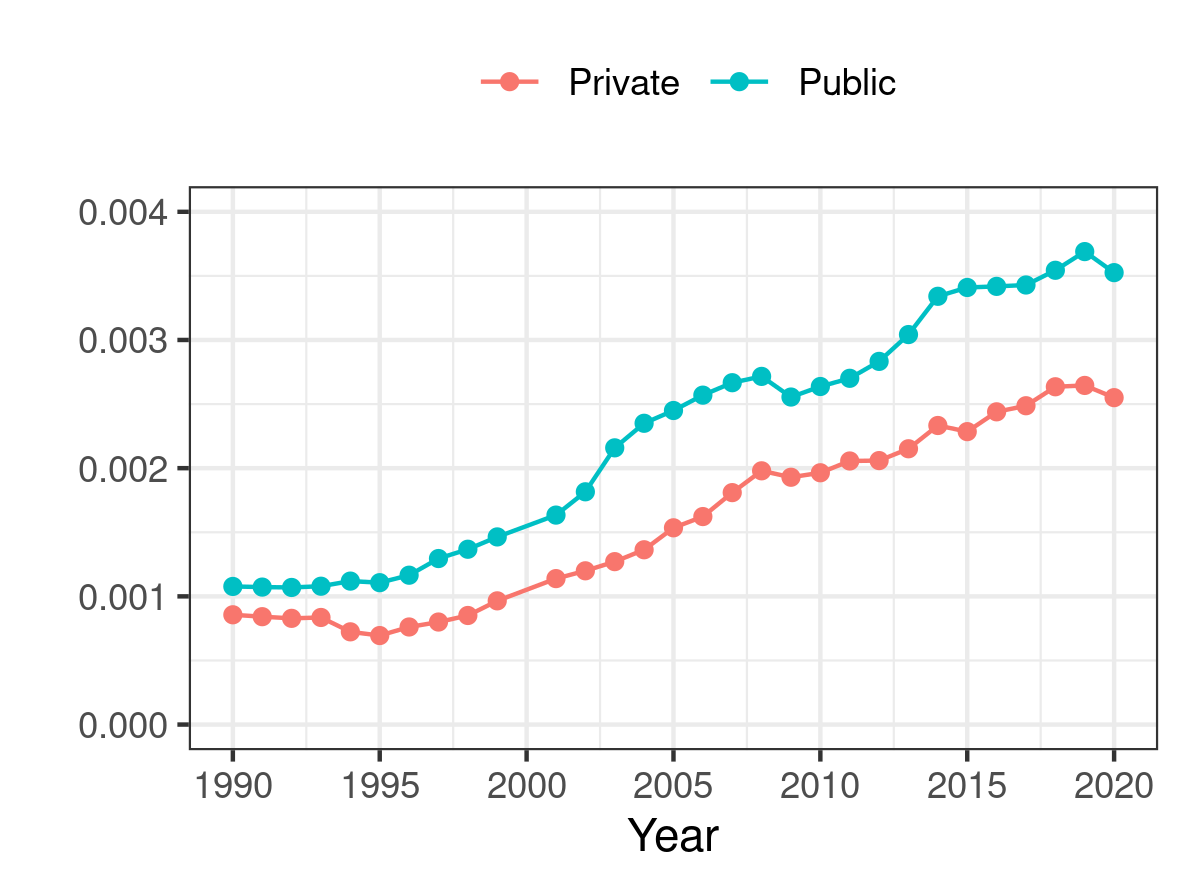
\includegraphics[width=\textwidth]{figures/lecturer-fte-perprof.png}
        \label{fig:lecturer-fte-perprof}
    \end{subfigure}
    \begin{subfigure}[b]{0.495\textwidth}
        \centering
        \caption{Assistant.}
        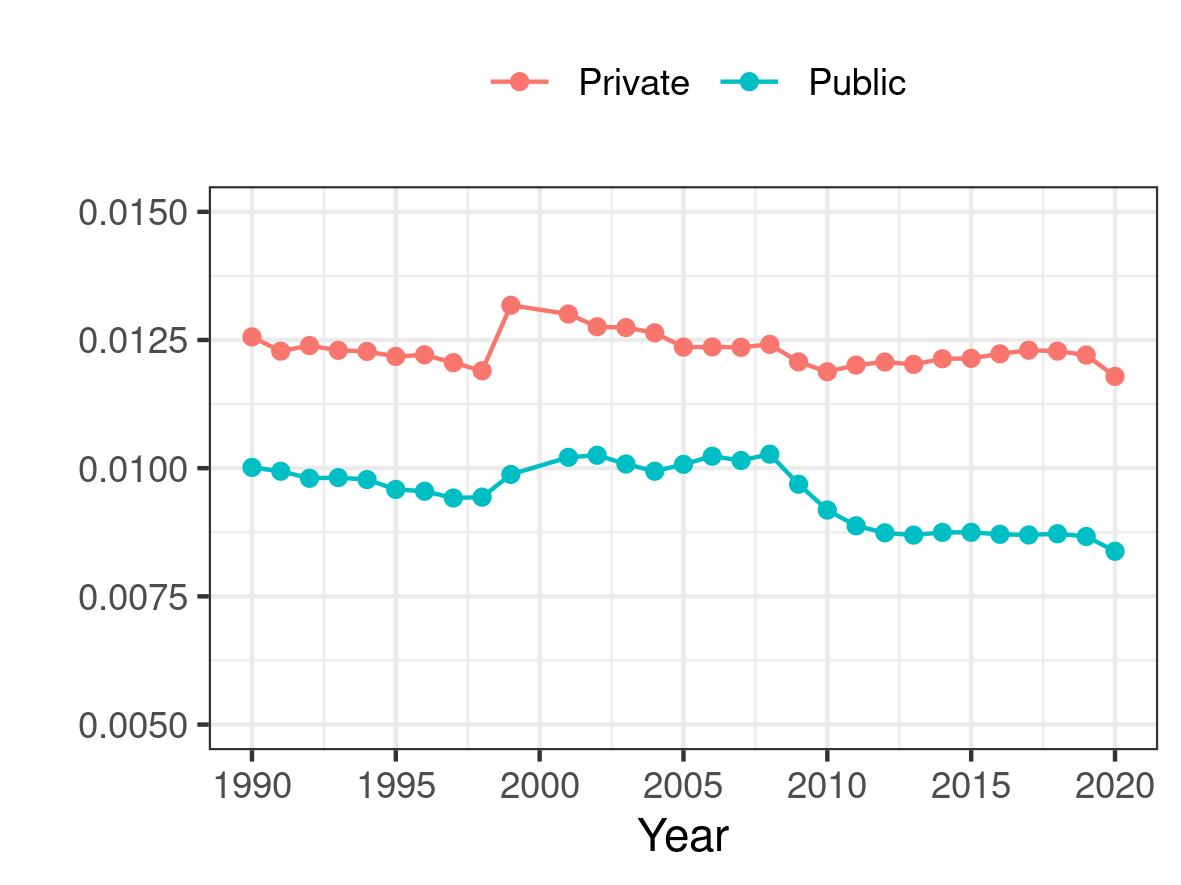
\includegraphics[width=\textwidth]{figures/assistant-fte-perprof.png}
        \label{fig:assistant-fte-perprof}
    \end{subfigure}
    \begin{subfigure}[b]{0.495\textwidth}
        \centering
        \caption{Full.}
        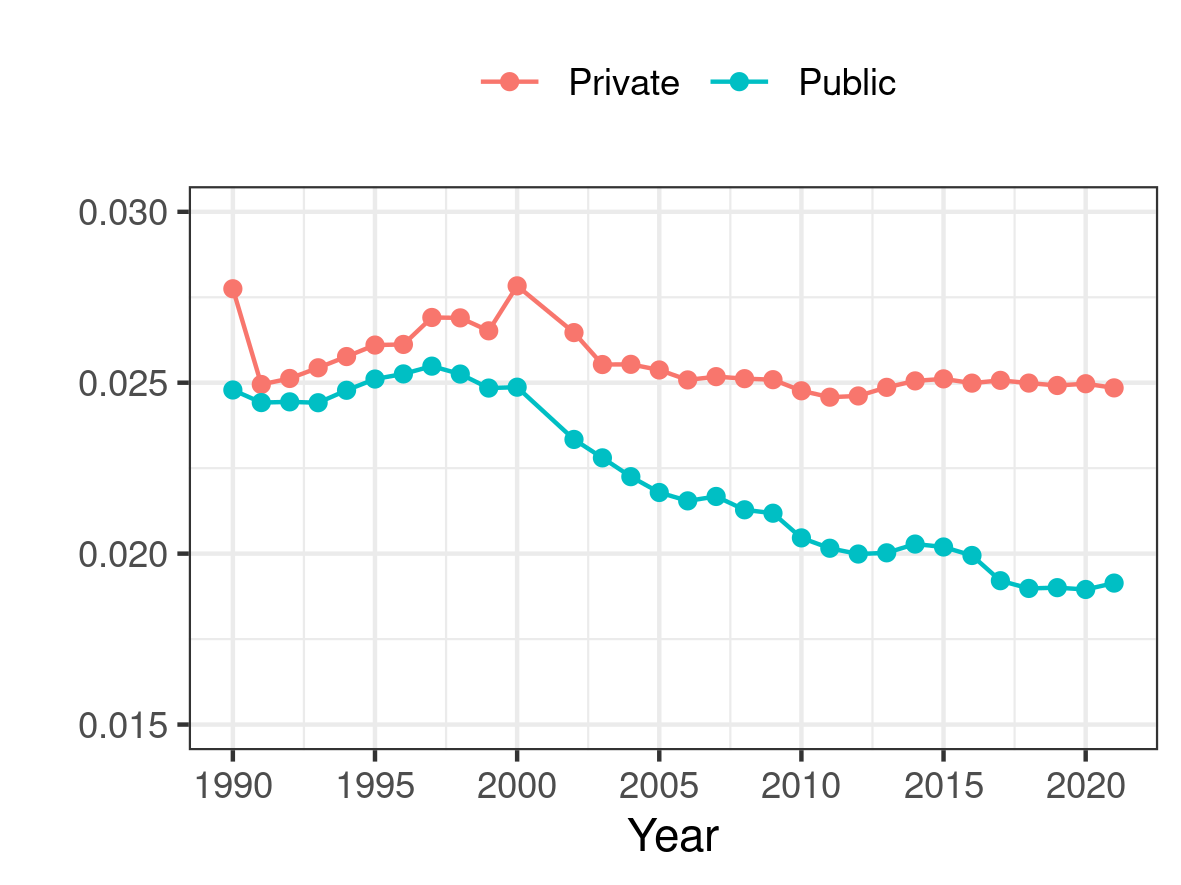
\includegraphics[width=\textwidth]{figures/full-fte-perprof.png}
        \label{fig:full-fte-perprof}
    \end{subfigure}
    \begin{subfigure}[b]{0.495\textwidth}
        \centering
        \caption{All.}
        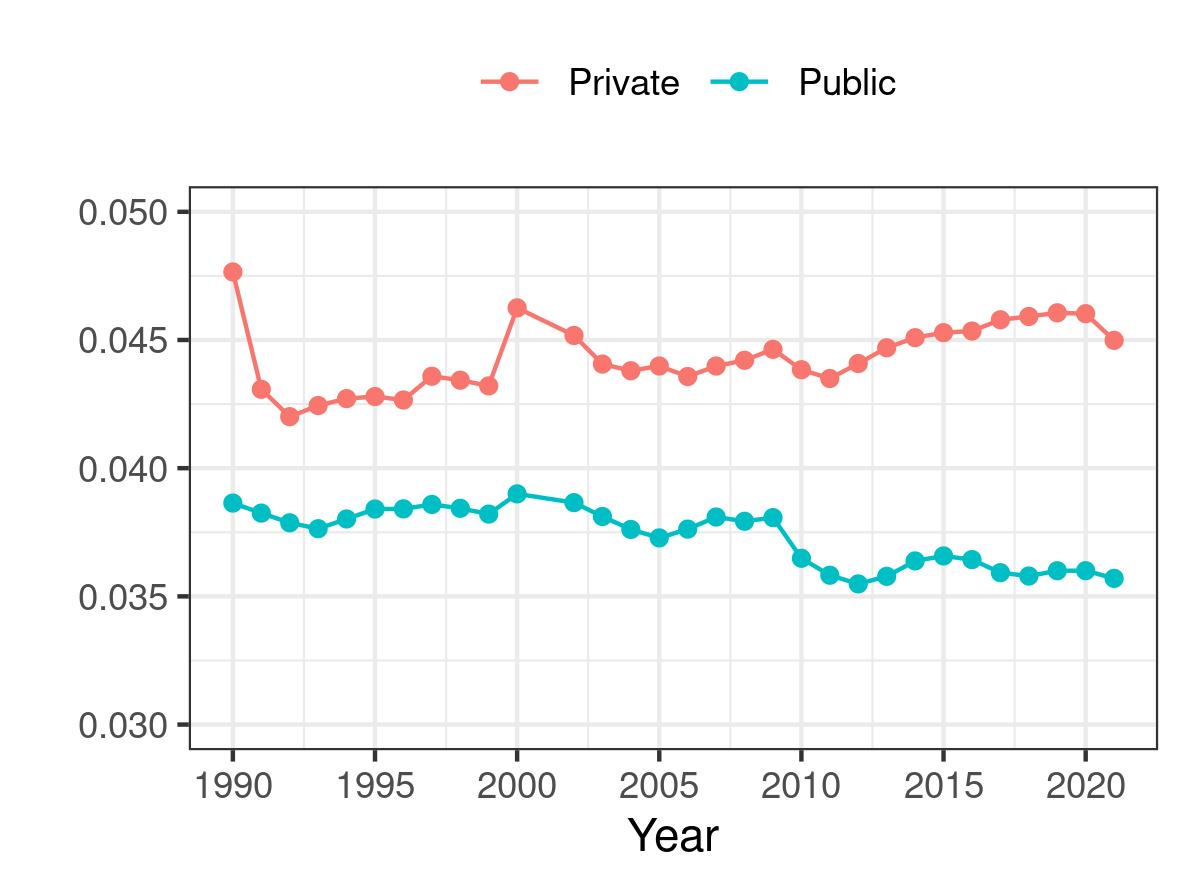
\includegraphics[width=\textwidth]{figures/all-fte-perprof.png}
        \label{fig:all-fte-perprof}
    \end{subfigure}
    \label{fig:fte-perprof}
\end{figure}

\autoref{fig:fte-perprof} documents the divergence in faculty composition (per student) between the average private and public university 1990-2021.
Private universities start with  a higher baseline of around 4.5 professors per 100 students, and exhibited yearly variation of less than 0.5 professor per hundred students over the thirty years.
Public universities start with 3.9 professors per hundred students, and this number falls to around 3.5 primarily in the 2008-2011 time period.
We see a similar difference in baseline, and fall for the years 2008-2011 for assistant professors.
Private and public universities have similar numbers of associated and full professors before the year 2000, yet this number has fallen by over 20\% in the next 20 years only for public universities: in 2021 the mean public university has 6 fewer full professors per hundred students than the mean private university.
Over the same time period, we see the rise in use of non-tenure track instructor positions (referred to as lecturers from here on), who were employed at similar rates in both sectors in 1990 yet have been utilised by public universities at a higher rate since.

\subsection{Trends in Illinois}
\label{sec:trends-illinois}

The state of Illinois experienced the same stagnation in state support for higher education that the rest of the nation has experienced 1990-2021.
\autoref{fig:illinois-funding} shows the trends for revenues among the seven Illinois public university campuses, including the falling share of state appropriations and substitution towards tuition revenue.

\begin{figure}[h!]
    \centering
    \singlespacing
    \caption{Mean Revenues among Illinois Public Universities, by Year.}
    \begin{subfigure}[b]{0.495\textwidth}
        \centering
        \caption{Total, millions \$ 2021 CPI-U.}
        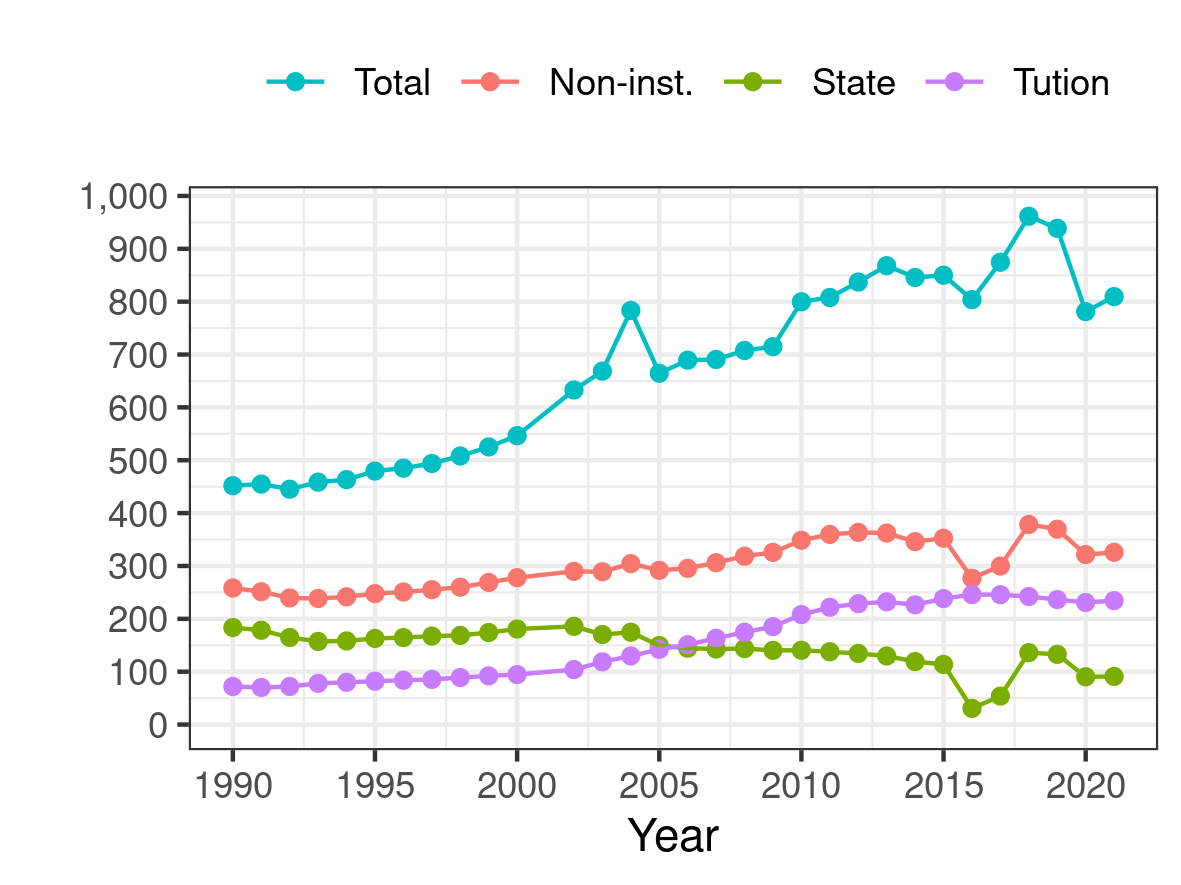
\includegraphics[width=\textwidth]{figures/illinois-funding-total.png}
        \label{fig:illinois-funding-total}
    \end{subfigure}
    \begin{subfigure}[b]{0.495\textwidth}
        \centering
        \caption{Per Enrolled Student, \$ 2021 CPI-U.}
        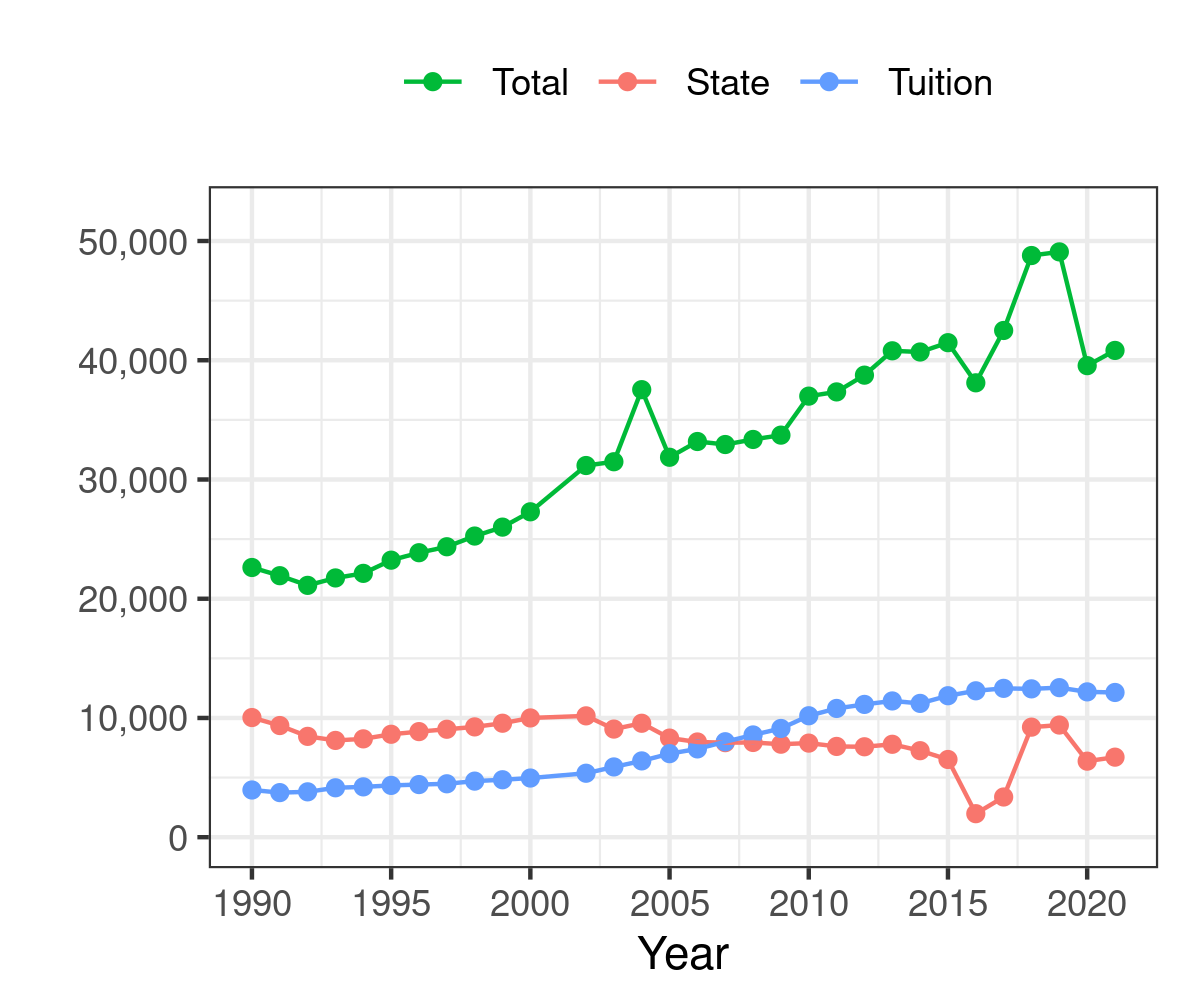
\includegraphics[width=\textwidth]{figures/illinois-funding-fte.png}
        \label{fig:illinois-funding-fte}
    \end{subfigure}
    \label{fig:illinois-funding}
\end{figure}

The decade of 2010-2021 has also seen yearly variation in its revenues, particularly around 2016.
In the calendar year 2015 partisan disagreements between the democratic legislature and republican governor led to the 2016 fiscal year starting with no state budget.
State agencies, and higher education institutions, employed accounting techniques to continue operating without any resources provided by the state government.\footnote{
    Fiscal year 2016 refers to June 205 to June 2016, as is the same for the academic year definition in this analysis. 
    K-12 schools were unaffected thanks to a separate budget agreement allowing non-higher education to operate as before.
}
While state institutions were able to stay open, there were drastic revenue and spending cuts in response to the budget impasse, as it continued through fiscal year 2017, and ended with a new budget restoring revenues to state agencies and universities for the 2018 fiscal year.
This variation in public university revenues via the state appropriations channel, stemming entirely from political disagreements --- not from state decisions regarding higher education and its finances \citep{young2020squandered} --- mean that Illinois public universities exhibit sizable changes in their state appropriations over 2010-2021, of similar order to those for the rest of the country over 1990-2021.

% Conceptual Framework
%%%%%%%%%%%%%%%%%%%%%%%%%%%%%%%%%%%%%%%%%
%% Section on possible outcomes
\section{Conceptual Framework}
\label{sec:conceptual}
%
%\textbf{Follow Prof Riehl's comments.
%    Also consider a theory toy-model where reach and teaching are plasuible substitutes, following \cite[Sec.~6.2]{NBERc13879}.
%    Better motivated if research spending is affected.
%}
%The, revenue shock induced, shift away from tenured profs may be mechanically relate to the shift between departments (towards STEM).
%Find a way to mix the “non-replacement of profs” with that for “department composition shift.”
%
%\subsection{University Responses to Financial Shocks}
%\label{sec:responses}

While state support for public higher education has stagnated at the same time as education costs rose, there are multiple possible ways that a university can respond.
\cite{NBERw23736} established that corresponding rises in tuition did not offset the falling state support, so that university spending (per student) fell in response to these persistent, negative state funding shocks.
There are multiple ways that these changes in finances may affect the faculty composition at public universities.

Universities every year hire a number of new professors, either to expand their departments or to replace leaving professors.
The number of professors hired is usually highest among non-tenured adjunct faculty, as these instructors are by majority hired on short-term contingent contracts, so that they are less costly to hire (or to not reinstate) in response to yearly changes in teaching needs.
Secondly, tenure-track assistant professors are hired in most years at public universities to replace leaving assistant professors, and are most often hired with a four to six year contract and agreement to be considered for tenure at the end of this term.
Lastly, tenured professors are those that have undergone review and have successfully secured a full-time appointment at their university with no expiration date; tenured professors may be hired from outside a university, though this position has the lowest hiring rate among most universities.
It is common for universities to restrict their faculty hiring in the face of financial shocks.
Since the yearly hiring rate is highest among lecturers and assistant professors, financial shocks may lower the number of lecturer and assistant professors at public universities the most, if faculty hiring is affected by falls in state funding.

Additionally, professors' salaries may be disrupted by the stagnation in public university finances.
When the university has a lower budget for its yearly hiring, it may respond by lowering the salary they offer to new hires.
This possible effect may not be the same across each position of professor; tenured faculty are often hired away from another university, so that new tenured professor hires could be less likely to accept a lower offer from a public university, and we would see that new tenured hires are not affected salary-wise.\footnote{
    \cite{blackaby2005} describes the academic outside options among economist faculty, documenting how they differ for academic position and gender.
}
Yet salary for all the professors, not just new hires, may also be affected: multiple universities passed a university-wide pay-cut for their faculty in response to state budget cuts around the 2008 recession, for example.\footnote{
    Indeed, Cornell University implemented both hiring freezes and even a nominal salary reduction for professors, in anticipation of a financial shock in early 2021.
    The salary cut was not permanent, as the oncoming financial shock turned out to not be as serious as projected, so that the salary cut was returned to professors in the year 2021.
}
Faculty are not paid the same by position, so that their are financial consequences for faculty being promoted between positions within a university.
In response to tightening fiscal restraints, universities may be less likely to grant tenure to assistant professors, or to promote tenured professors from associate to full professor either.

It is not immediately clear which effect will dominate, and which position of professor will be effected the most by changes in their university's finances.
Yet, there is one empirical fact worth noting: a mean assistant or tenured professor earns more than double that of an adjunct lecturer per year (\autoref{tab:illinois-summary}), and the tenure contract means universities are compelled to pay that higher salary for more years than contingent lecturers.
If a public university's primary obligation is to teach, and they must fulfil this objective with fewer and fewer resources, then they may substitute away from tenure-track and tenured professor towards contingent lecturers to achieve this obligation.\footnote{
    That is substituted away from tenure-track and tenured professors according to the salary ratio, and the relative productivity between these two positions.
    It is not possible to estimate the relative productivity in this paper, so I leave the rate of substitution between the two positions to further research.
}

% Empirical methods
%%%%%%%%%%%%%%%%%%%%%%%%%%%%%%%%%%%%%%%%%
%% Empirical section
\section{Empirical Framework}
\label{sec:empirics}

A professor is employed by a university, so it stands to reason that when public universities experience a secular fall in one of their revenue sources revenue --- analogous to a demand shock in the private sector --- that the composition of their employees will be affected.

Na\"ively we can analyse the relationship between professor-outcomes $Y_{i,t}$ at university $i$ in year $t$ as a result of state funding per student $X_{i,t}$.
Outcomes include count of professors per student within each university-year.
This model gives $\beta$ the association with these outcomes and state funding per student,\footnote{
    Note that dividing by student count also implicitly controls for the size of the university, so that this model accounts for yearly variation in professor count and university revenues arising from growth in a university.
}
including fixed effects to control for effects specific to the university and year.
Log$(.)$ transforming the variables improves the interpretability of $\beta$ as an elasticity for professor count per student with respect to state funding per student.
\begin{equation}
    \label{eqn:naivereg}
    Y_{i,t} = \alpha_i + \gamma_t + \beta X_{i,t} + \epsilon_{i,t}
\end{equation}

Yet a university's finances are not exogenous to state decisions for support of higher education, or exogenous to internal institutional decisions.
Instead, the state government and university administration undertake a complex process of allotting resources across multiple different priorities, including instruction, research, or between departments.
Importantly for this analysis, revenues received from an institution's state government provide opportunity to address this endogeneity.


\subsection{State Appropriation Shocks}
\label{sec:approp-shocks}

\cite{NBERw23736,chakrabarti2018effect,NBERw27885} address endogeneity in public university finances by exploiting a shift-share instrument for changes in state-level funding interacted with university reliance on state funding in a base period.
\begin{align}
    \label{eqn:public-instrument}
    Z_{i,t} &\coloneqq - \log \left[
    \left( \frac{\text{Total State Funding}_{s(i),t}}{\text{Student Population}_{s(i),t}} \right)
    \sum_{\tau = 0}^{3} \frac 14
    \left( \frac{\text{State Funding}_{i,1990 + \tau}}{\text{Total Revenues}_{i,1990 + \tau}} \right) \right]
\end{align}
The system exploits the fact that institutions who rely on state appropriations more will be affected by state appropriation shocks.
$Z_{i,t}$ is the instrument for (log) state appropriations for institution $i$ in year $t$, interacting the average funding for universities in state $s(i)$ with reliance on state funding relative to total revenues, averaged across the base years 1990--1993.\footnote{
    1990--1993 are defined as data for public university finance data are most comparable (i.e. without many missing values) beginning in 1990.
    \cite{NBERw23736} use the single year 1990 as the base year, though I use the four years to ameliorate missing values in the single year of 1990.
    Results are similar in either specification.
}
$Z_{i,t}$ is contructed as negative to reflect the fact that the long term trend in, and most of the short-run shocks to, state funding for higher education has been negative.
State funding has been been falling, so that the instrument describes shocks to university revenues, mostly in a negative direction.

\cite{NBERw27885} notes the tendency for public universities to respond to state funding cuts by increasing reliance on tuition, where \cite{NBERw23736} specifically instruments for tuition revenues with collected information on legislative tuition price controls.\footnote{
    \label{foot:control}
    It may be argued that tuition revenues are confounder between the causal effect of changes in state funding on a university's total revenues, so that this analysis focuses on state support for higher education (no total revenue) as a result.
    This follows the \cite{NBERw27885} formulation.
    On the other hand, rises in tuition revenues (per student) may arise as result of tuition hikes thanks declining state support, which would mean controlling for tuition would constitute a bad control.
    Estimates including tuition revenues (per student) as a control in the second stage of the IV estimates produces results of very similar magnitude and direction, and so are omitted.
}
This analysis focuses on one important source of revenues for public universities: state appropriations.

The first-stage is then as follows, including institution and year fixed effects.
\begin{equation}
    \label{eqn:firststage}
    X_{i,t} = \eta_i + \zeta_t + \delta Z_{i,t} + \epsilon_{i,t}
\end{equation}
We note the conditions for exogeneity in the instrument (following the discussion presented by \citealt{NBERw27885}).
The instrument is exogenous if state policy decisions for funding of public universities are uncorrelated with unobserved institutional changes of any specific college or university in the state \citep{borusyak2022quasi}.
This assumption is plausible given that the majority of states have multiple (i.e. more than five) public universities, without any single university campus receiving the majority of state funding within any single state.
Secondly, addressing endogeneity in university revenues by the shift-share identification strategy requires exogeneity in either the base-line share or shift component of the instrument.
In this case, we satisfy the second: universities' institutional-level decisions are not correlated with contemporaneous or upcoming shocks to state appropriations.\footnote{
    It would be plausible to consider the case that universities make institutional-level decisions in a consistently different manner to those 
    with differing reliance on state appropriations in 1990, so that exogeneity by the base-line share is not plausible here.
}

\begin{table}[h!]
    \singlespacing
    \centering
    \caption{First Stage Estimates, for State Funding by Appropriation Shock.}
    \makebox[\textwidth][c]{
\begin{tabular}{@{\extracolsep{5pt}}lcccc} 
\\[-1.8ex]\hline 
\hline \\[-1.8ex] 
 & \multicolumn{4}{c}{Dependent Variable: Non-institutional Revenues} \\ 
\cline{2-5} 
\\[-1.8ex] & (1) & (2) & (3) & (4)\\ 
\hline \\[-1.8ex] 
 Appropriations Shock & 0.990 & 0.608 & 0.980 & 0.350 \\ 
  & (0.075) & (0.059) & (0.078) & (0.084) \\ 
  Tuition Revenue & 0.063 & 0.558 &  &  \\ 
  & (0.055) & (0.059) &  &  \\ 
  Constant &  & $-$0.982 &  & 6.011 \\ 
  &  & (0.751) &  & (0.688) \\ 
 \hline \\[-1.8ex] 
Uni. + Year fixed effects? & Yes & No & Yes & No \\ 
F stat. & 92.461 & 88.72 & 156.791 & 17.487 \\ 
Observations & 18,504 & 18,504 & 18,504 & 18,504 \\ 
R$^{2}$ & 0.801 & 0.222 & 0.801 & 0.064 \\ 
\hline 
\hline \\[-1.8ex] 
\end{tabular} 
}
    \label{tab:firststage-reg}
    \begin{flushleft}
        \footnotesize
        \textbf{Note}: Standard errors are clustered at the state-year level.
    \end{flushleft}
\end{table}

\autoref{tab:firststage-reg} presents results of the first-stage regression, separately with and without a control for tuition revenue per student, plus institution and year fixed effects.\footnote{
    Representations for frequentist significance levels (i.e. 10, 5, 1\% etc.) are omitted here, and in all following tables.
}
We note columns (1) and (2) estimate that a shock to appropriations (per student in the entire state) of 10\% is associated with 9.8\% change in state funding per student at the university; the instrument is strong, and we note similarity in estimates with and without inclusion of fixed effects.
Columns (3) and (4) include the tuition revenue control (explained in \autoref{foot:control}) to exhibit estimates with the inclusion of this possible collider or bad control.
Column (3) shows similar estimates to columns (1), (2) thanks to inclusion of fixed effects, so that the fixed effects was effective in soaking variation in per-student tuition revenues at the institution-year level.
Column (1) represents the estimates for \autoref{eqn:firststage} with fixed effects, omitting the tuition revenue control, and is the preferred form that I proceed with in the following.

\begin{figure}[h!]
    \centering
    \singlespacing
    \caption{Local Projection Estimates for First-Stage \autoref{eqn:firststage}.}
    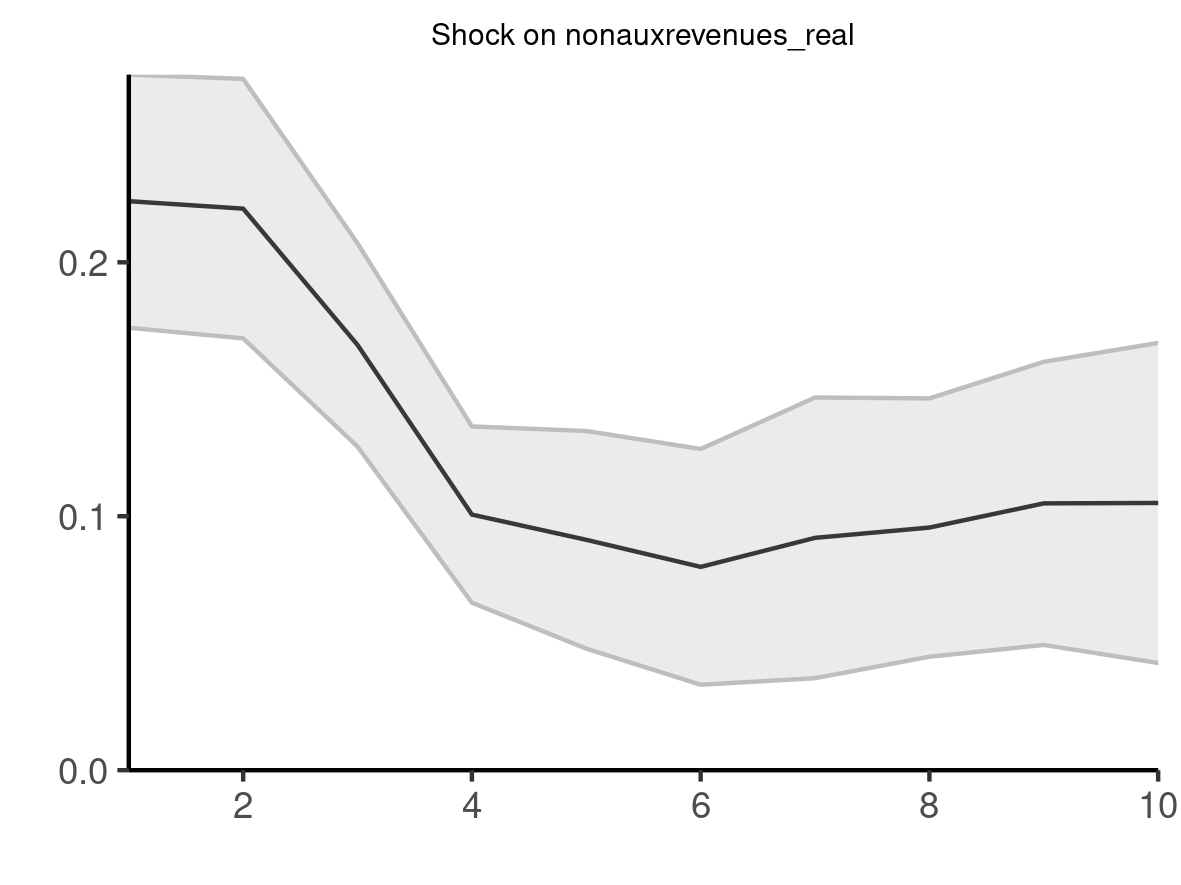
\includegraphics[width=0.6\textwidth]{figures/firststage-lp.png}
    \label{fig:firststage-lp}
\end{figure}

\autoref{fig:firststage-lp} presents local projection estimates for the staying-power of the state appropriation shock to university revenues, with each year showing the years following effect of a shock to state reveunes in year zero.
We see a decaying, yet real and positive, effect of the shock on revenues for the next 10 years, illustrating that the state appropriation shock is a strong, if fading, instrument for state funding per student and justifying its use in local projection IV estimation.

These results, together with the case for exogeneity, show the appropriations shock instrument strongly predicts university revenues in the first-stage estimation.


\subsection{Instrumental Variables Model, University-Level}
\label{sec:iv-model-uni}

The primary empirical model combines the instrumental variable for state appropriation shocks with the empirical model for the effects of state funding at the university-level --- i.e. parameter $\beta$ in the following.\footnote{
    It is important to note the treatment effect isolated here; the instrumental variables approach identifies the local average treatment effects (LATE) specific to the instrument.
    So we interpret this treatment effect as a university's response in employment count and average salaries to state funding changes, changes specific to state appropriation shocks, among the complier group --- i.e. universities with any exposure to shocks, assuming no universities increase employment or salaries in response to negative revenue shocks.
    \cite{mogstad2021causal} provide a full discussion of the LATE with instruments and multiple monotonicity conditions.
}
\begin{eqnarray}
    \label{eqn:secondstage1}
    X_{i,t} &=& \eta_i + \zeta_t + \delta Z_{i,t} + \epsilon_{i,t} \\
    \label{eqn:secondstage2}
    Y_{i,t} &=& \alpha_i + \gamma_t + \beta \widehat X_{i,t} + \varepsilon_{i,t}
\end{eqnarray}
I estimate the system by two stage least squares, including institution and year fixed effects, and investigate outcomes at the university-level to analyse effects on the university as a result of changes in revenues.
Additionally, I estimate the model via local projections \citep{jorda2005,miller2022} to investigate whether the effects of revenues on faculty composition linger for multiple years after the original appropriation shock.
Regarding outcomes, I focus on the composition of the professors employed at the university by analysing (log) count per student, and average salaries paid to, professors employed by the university.

\begin{figure}[H]
    \centering
    \singlespacing
    \caption{Instrument Variables Model for University Finances and Faculty Composition.}
    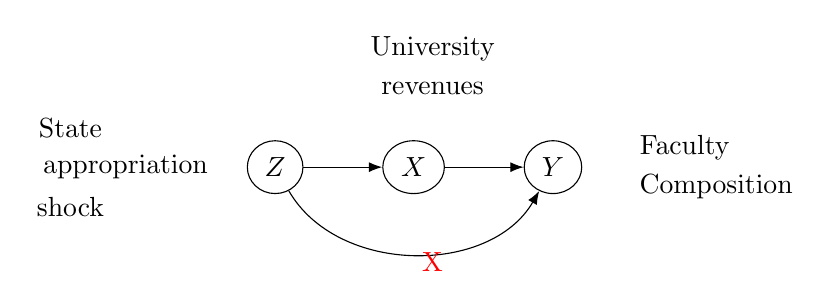
\begin{tikzpicture}
        \node[state] (instrument) at (0,0) {$Z$};
        \node at (-2.6,0.5){State};
        \node at (-1.9,0){appropriation};
        \node at (-2.6,-0.5){shock};
        \node[state] (endogenous) [right=of instrument] {$X$};
        \node at (2,1.5) {University};
        \node at (2,1) {revenues};
        \node[state] (outcome) [right=of endogenous] {$Y$};
        \node at (5.2,0.25) {Faculty};
        \node at (5.6,-0.25) {Composition};
        % Relevance condition
        \path (instrument) edge (endogenous);
        \path (endogenous) edge (outcome);
        % Exclusion Restriction
        \path (instrument) edge[bend right=60] (outcome);
        \node[color=red] at (2,-1.2) {X};
    \end{tikzpicture}
    \label{fig:SCM-ivmodel}
\end{figure}

\autoref{fig:SCM-ivmodel} presents the system in graphical form, for the causal effect of state appropriation shocks on university revenues and thus faculty composition, making clear the assumption that appropriation shocks affect faculty composition only via affecting university finances.


\subsection{Instrumental Variables Model, Individual Professor-Level}
\label{sec:iv-model-indiv}

This analysis additionally uses data regarding individual professors in the Illinois university system, to investigate the effects of changes in university revenues on the individual professors at the universities.
Redefining the level of outcome requires adjustment to the empirical approach, leveraging variation in university finances for the years after a professor joins the university.\footnote{
    This formulation follows that presented by \cite{NBERw27885}, where individual student outcomes are analysed via variation in state appropriations after their freshman-year.
    This contrasts with \autoref{sec:iv-model-uni} and \cite{NBERw23736}, where the unit of analysis is the university-year.
}

\autoref{eqn:rolling-instrument} defines a rolling-share variant of the instrument, $\tilde Z_{j,t}$, where the university's state appropriations share exposure is based in the year a professor joins the university --- and not the base period 1990--1993.
$j$ indexes each professor in year $t$, $\tau(j)$ for the year the professor first joins their institution.\footnote{
    Identifying $\tau(j)$ is possible for $j$ by restricting to all professors hired 2011-2021 --- i.e. in the years after the start of the full panel.
    It is not possible to discern the hiring year for professors who  were hired in the years preceding 2011, and so the entire sample is only possible to analyse using the base-share in years 1990-1993 formulation (e.g., \autoref{tab:facultysalaries-shock-illinois}, \ref{tab:promotion-shock-illinois}).
}
\begin{align}
    \label{eqn:rolling-instrument}
    \tilde Z_{j,t} &\coloneqq - \log \left[
    \left( \frac{\text{Total State Funding}_{s(j),t}}{\text{Student Population}_{s(j),t}} \right)
    \left( \frac{\text{State Funding}_{\tau(j)}}{\text{Total Revenues}_{i,\tau(j)}} \right) \right]
\end{align}

This approach leverages an insight, made available by level of the data: that an individual professor is affected by changes in university revenues after they have joined the university.\footnote{
    Notice that \autoref{sec:iv-model-uni} considers the number of professors employed by the university; whether a professor becomes employed at the university is likely affected by that university's finances.
    The formulation in this section does not consider whether the professor joins the university, instead taking as given that the professor is employed at the university, and then projects the effect on the individual.
}
Exogeneity and relevance of the rolling-share instrument, $\tilde Z_{j,t}$, follows the same reasoning as that for the base-share instrument, $Z_{i,t}$, discussed in \autoref{sec:approp-shocks}.\footnote{
    The base-share instrument is appropriate for some outcomes with the individual Illinois professors, where appropriate (\autoref{tab:facultysalaries-shock-illinois}, \ref{tab:promotion-shock-illinois}).
}
We satisfy the assumptions for exogeneity by noting that none of the Illinois public campuses take the majority of state appropriations, and that the instrument identification strategy relies on exogeneity in changes in state appropriations to individual professor-outcomes, following the year they joined the university.\footnote{
    Additionally, within-institution changes resulting from share reliance on state funding may be correlated with unobserved changes in the outcomes, so that \cite{NBERw27885} note the importance of controlling for the base share and state student population.
    The formulation here implicitly controls for these factors via the fixed effects; results are relatively similar while including these controls without including fixed effects, and so are omitted.
}
\autoref{tab:firststage-illinois} presents results of the first stage estimation, showing that the instrument is strong in the same way as that for the university-level outcomes (\autoref{tab:firststage-reg}), with very similar estimates for the association between appropriation shocks and non-institutional revenues.

The instrumental variables model is then defined as follows where $i(j)$ refers to the institution that professor $j$ is employed at, and $Y_{j,t}$ refers to individual-level outcomes total salary, rate of promotion, and propensity to leave the Illinois public university system.
The system includes a fixed effect for the institution and first year of employment.\footnote{
    The instrument varies by institution, based in the year of first employment, so that these are the corresponding fixed effects and levels of clustered standard errors.
}
\begin{eqnarray}
    \label{eqn:secondstage1_indiv}
    X_{i(j),t} &=& \theta_{i(j)} + \phi_{\tau(j)} + \delta \tilde Z_{i(j),t} + \epsilon_{i(j),t} \\
    \label{eqn:secondstage2_indiv}
    Y_{j,t} &=& \mu_{i(j)} + \nu_{\tau(j)} + \beta \widehat X_{i(j),t} + \varepsilon_{j,t}
\end{eqnarray}
We then interpret parameter $\beta$ as the effect of changes in state funding at an Illinois public university, via state appropriation shocks, on an individual professor's outcome $Y_{j,t}$.

% Empirical results
%%%%%%%%%%%%%%%%%%%%%%%%%%%%%%%%%%%%%%%%%
%% Results section
\section{Results}
\label{sec:results}

\subsection{University-Level}

\autoref{tab:facultycount-shock-reg} presents OLS and IV estimates, where the outcome is (log) count of professors employed at the university, separated by position, and for all professors (Columns 7, 8).
For all professors we see a positive correlation between university revenues and professor count per student (the OLS columns), where an increase in university total revenues by 10\% is associated with an increase in professor count per student of 0.83\%, yet negatively correlated with lecturer count of -1.3\%.
Lecturers per student is not shown to be correlated with total university revenues.
The 2SLS columns show results after identifying state funding with the appropriation shock.
All professor count per student increases by 0.53\% in response to a 10\% rise in total revenues.
The effect is driven by increases in the count of assistant and full professors (i.e. tenure-track and tenured) per student, where assistant professor count per student increase by 1.4\%, and full professor 1.2\%.
The count of lecturers per student decreases by 4.4\% in response to a (positive) 10\% shock in university revenues.

\begin{table}[h!]
    \singlespacing
    \centering
    \caption{OLS and 2SLS Estimates for University Faculty Composition.}
    \makebox[\textwidth][c]{
\begin{tabular}{@{\extracolsep{5pt}}lcccccccc} 
\\[-1.8ex]\hline 
\hline \\[-1.8ex] 
 & \multicolumn{8}{c}{Dependent Variable: Employment Count by Professor Group} \\ 
\cline{2-9} 
\\[-1.8ex] & \multicolumn{2}{c}{Lecturer} & \multicolumn{2}{c}{Assistant} & \multicolumn{2}{c}{Full} & \multicolumn{2}{c}{All} \\ 
 & OLS & 2SLS & OLS & 2SLS & OLS & 2SLS & OLS & 2SLS \\ 
\\[-1.8ex] & (1) & (2) & (3) & (4) & (5) & (6) & (7) & (8)\\ 
\hline \\[-1.8ex] 
 Non-inst. Revenues & $-$0.059 & $-$1.426 & 0.348 & 0.659 & 0.453 & 0.530 & 0.360 & 0.310 \\ 
  & (0.162) & (0.590) & (0.126) & (0.207) & (0.154) & (0.134) & (0.144) & (0.100) \\ 
  Tuition Revenue & 0.432 & 0.951 & 0.091 & $-$0.028 & $-$0.060 & $-$0.090 & 0.040 & 0.059 \\ 
  & (0.103) & (0.234) & (0.098) & (0.101) & (0.080) & (0.065) & (0.061) & (0.053) \\ 
 \hline \\[-1.8ex] 
Observations & 17,329 & 17,329 & 17,826 & 17,826 & 17,929 & 17,929 & 18,504 & 18,504 \\ 
R$^{2}$ & 0.673 & 0.631 & 0.720 & 0.712 & 0.794 & 0.793 & 0.827 & 0.827 \\ 
\hline 
\hline \\[-1.8ex] 
\end{tabular} 
}
    \begin{flushleft}
        \footnotesize
        \textbf{Note}: Standard errors are clustered at the state-year level.
    \end{flushleft}
    \label{tab:facultycount-shock-reg}
\end{table}

\autoref{fig:all-count-lp} shows local projection estimates, where the effect on total professor count per student persists at the same magnitude of around 0.1 four years after the identified shock.
These findings are in line with \cite{turner2014impact} observing that universities froze hiring particularly for tenure-track positions in response to negative budget shocks in the late 2000s, and \cite{brown2014endowment} from shocks to university endowments.
We see a negative coefficient for the number of lecturers per student.
This effect lines up with two trends we see in \autoref{sec:trends}: that public universities revenues (per student) are decreasing while utilisation of non-tenure track lecturers increased over the same time period.
And yet, identifying the university revenues by the state appropriations shock increases the magnitude of the effect (Column 2) with respect to the association (Column 1), strengthening the case that the two trends are causally linked.
Between years 1990-1999 IPEDS provided count of professors by explicit tenure designation (opposed to named position as in \autoref{tab:facultycount-shock-reg}), and \autoref{tab:tenurecount-shock-reg-fte} presents results of the respective regressions by tenure status.
Results are relatively similar, yet imprecise from the much smaller number of observations.

Together these findings show that public universities increase (decrease) their count of tenure-track and tenured professors per student in years when revenues are more (less) plentiful, possibly by increasing hiring intensity or efforts to maintain incumbent professors.
In the same vein, when revenues are (not) bountiful, count of tenure-track and tenured professors per student increases (decreases).
%Yet, further analysis is needed to disentangle the possible long-run effects of state revenues on faculty composition among public universities.

\subsection{Long-term Effects on Faculty Composition}

\begin{figure}[h!]
    \centering
    \singlespacing
    \caption{Local Projection Estimates for Professor Count per Student, by Professor Group.}
    \begin{subfigure}[b]{0.495\textwidth}
        \centering
        \caption{Lecturers.}
        \includegraphics[width=\textwidth]{figures/lecturer-count-lp.png}
        \label{fig:lecturer-count-lp}
    \end{subfigure}
    \begin{subfigure}[b]{0.495\textwidth}
        \centering
        \caption{Assistant Professors.}
        \includegraphics[width=\textwidth]{figures/assistant-count-lp.png}
        \label{fig:assistant-count-lp}
    \end{subfigure}
    \begin{subfigure}[b]{0.495\textwidth}
        \centering
        \caption{Full Professors.}
        \includegraphics[width=\textwidth]{figures/full-count-lp.png}
        \label{fig:full-count-lp}
    \end{subfigure}
    \begin{subfigure}[b]{0.495\textwidth}
        \centering
        \caption{All Professors.}
        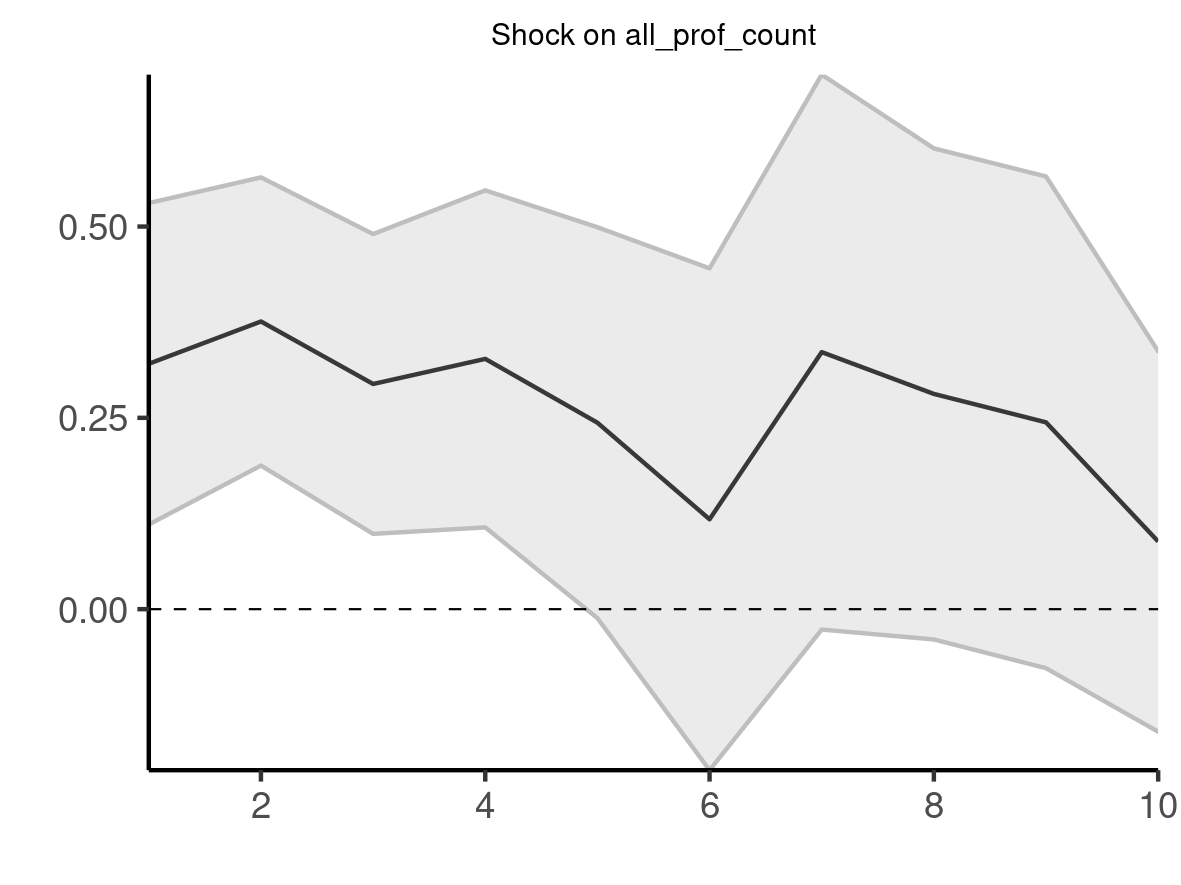
\includegraphics[width=\textwidth]{figures/all-count-lp.png}
        \label{fig:all-count-lp}
    \end{subfigure}
    \label{fig:count-lp}
\end{figure}

Decreases in university revenues (via state funding shocks) affect faculty composition for at most 4 years after the initial revenue shock.
A 10\% decrease in state funding increases count of lecturers per student by 4\% for the first two years after the initial shock.
While count of assistant professors decreases 10 to 18.5\% three years later;
count of tenured professors decreases 9 to 6\% three years later.
Together, the total count of professors per student decreases around 1\% for three years after the initial funding shock, and the effect is not distinguishable from zero four years after.

\autoref{fig:count-lp} represents these estimates, using the local projection method, as a series of impulse responses for each outcome of professor count.
The mechanism that explains the changes in faculty composition are, however, not clear at this unit of analysis; individual data are needed to delve deeper.

\subsection{Individual Professor Outcomes}

I first examine whether a shock to the university's revenues affects the salaries of professors at the university.
The first outcome is first-year salary for each professor by their position;
\autoref{tab:newhiresalaries-shock-illinois-rolling} presents 2SLS estimates for the elasticity of total salaries with respect to university revenues, among the sample with a year of starting employment after 2010.
New hires of assistant, full, or administrative position professors are not related to revenues, via a shock to appropriations in their first-year of employment.
Yet, the starting salary of lecturers is 3.8\% higher given an increase in their hiring university's state funding of 10\%.

\begin{table}[h!]
    \singlespacing
    \centering
    \caption{2SLS Estimates for Faculty Salaries, in First-Year, at Illinois Universities.}
    \makebox[\textwidth][c]{
\begin{tabular}{@{\extracolsep{5pt}}lccccc} 
\\[-1.8ex]\hline 
\hline \\[-1.8ex] 
 & \multicolumn{5}{c}{Dependent Variable: Salaries by Professor Group} \\ 
\cline{2-6} 
 & Lecturer & Assistant & Full & Admin & All \\ 
\\[-1.8ex] & (1) & (2) & (3) & (4) & (5)\\ 
\hline \\[-1.8ex] 
 State Funding & 0.384 & $-$0.256 & $-$0.378 & $-$0.130 & 0.238 \\ 
  & (0.158) & (0.212) & (0.313) & (0.331) & (0.196) \\ 
 \hline \\[-1.8ex] 
Observations & 8,786 & 5,090 & 1,248 & 3,153 & 18,277 \\ 
R$^{2}$ & 0.303 & 0.075 & 0.100 & 0.250 & 0.223 \\ 
\hline 
\hline \\[-1.8ex] 
\end{tabular} 
}
    \begin{flushleft}
        \footnotesize
        \textbf{Note}: Standard errors are clustered at the institution and first year of employment level. 
    \end{flushleft}
    \label{tab:newhiresalaries-shock-illinois-rolling}
\end{table}

Regarding total salary for every year of employment, \autoref{tab:facultysalaries-shock-illinois-rolling} presents estimates for the elasticity of total salary with respect to university revenues, for the entire sample of professors hired after 2010.\footnote{
    Recall that this is a subsample of the entire data, that the rolling shift-share instrument is only defined for the sample with an observed hiring date in the years 2011-2021.
}
The elasticity is non-distinguishable from zero among any position, implying that long-term salaries are not related to state funding.
\autoref{tab:facultysalaries-shock-illinois} presents the same model, for the sample of all professors and using the instrument based in years 1990-1993, similarly finding no relationship.

\begin{table}[h!]
    \singlespacing
    \centering
    \caption{2SLS Estimates for Faculty Salaries at Illinois Universities.}
    \makebox[\textwidth][c]{
\begin{tabular}{@{\extracolsep{5pt}}lccccc} 
\\[-1.8ex]\hline 
\hline \\[-1.8ex] 
 & \multicolumn{5}{c}{Dependent Variable: Salaries by Professor Group} \\ 
\cline{2-6} 
 & Lecturer & Assistant & Full & Admin & All \\ 
\\[-1.8ex] & (1) & (2) & (3) & (4) & (5)\\ 
\hline \\[-1.8ex] 
 Non-inst. Revenues & 0.009 & $-$0.072 & $-$0.044 & $-$0.013 & $-$0.011 \\ 
  & (0.094) & (0.040) & (0.038) & (0.049) & (0.086) \\ 
 \hline \\[-1.8ex] 
Observations & 25,820 & 22,156 & 9,001 & 11,472 & 68,449 \\ 
R$^{2}$ & 0.217 & 0.051 & 0.074 & 0.143 & 0.161 \\ 
\hline 
\hline \\[-1.8ex] 
\end{tabular} 
}
    \begin{flushleft}
        \footnotesize
        \textbf{Note}: Standard errors are clustered at the institution-year level.
    \end{flushleft}
    \label{tab:facultysalaries-shock-illinois-rolling}
\end{table}

Note that professor position (assistant, associate, full) is also an outcome, thanks to the promotion channel: a university may be less able to promote their professors to higher paying positions when their revenues are constrained.
\autoref{tab:promotion-shock-illinois-rolling} shows estimates where the outcome is rate of promotion within each professor position.
The lecturer position describes the sample of professors who were ever listed as a non-tenure track lecturer and the binary for promotion equals one in a year they achieved an assistant professor position; assistant the same for the assistant to associate professor promotion; associate same for associate to full promotion.
There is no discernible relationship between revenues and promotion among any position.\footnote{
    \autoref{tab:promotion-shock-illinois} shows estimates using the base-year instrument among the entire sample, finding the same results.
}
Furthermore, local projection estimates (\autoref{fig:promoted-illinois-lp}) show that the there is no promotion effect, among all professors, for any of the following years either.
Lastly, \autoref{tab:facultyleaving-shock-illinois-rolling}, \ref{tab:facultyleaving-shock-illinois} describes estimates for rate of exit from the employing university among Illinois professors, and finds no relationship with university revenues.

% Dicussion
%%%%%%%%%%%%%%%%%%%%%%%%%%%%%%%%%%%%%%%%%
%% Discussion section
\section{Discussion}

The results show that the recent stagnation in state funding for higher education has affected the composition of faculty within public universities, away from tenure-track and tenured professors towards non-tenured lecturers.
At the same time, there are little discernible effects on individual professors hired in the years 2011-2021 at Illinois public universities, except for the salaries of first year lecturers.
The rate that faculty leave their university, and their rate of promotion between positions, are unaffected by the university revenues, so this leaves one primary channel to explain changes in faculty composition: hiring.

\cite{turner2014impact} documents the wide-spread practice of hiring freezes at universities in response to budget shocks around the 2008 recession.
Throughout the last decade, multiple such measures were taken by Illinois public universities in response to their deteriorating finances \citep{furlough2010}.
The University of Illinois\footnote{
    The University of Illinois includes three public university campuses: Urbana-Champaign, Chicago, Springfield.
}
did not receive the allocated state appropriations from the state of Illinois on time, so enacted cost-cutting measures to stay fiscally solvent.
The university system placed a hold on all hiring for filling state-funded positions and promotions.
Faculty were furloughed (placed on leave without pay) for a day each month, and university administrators placed on two days per month furlough, or eligible university employees could accept a voluntary, equivalent pay reduction.
The University of Western Illinois adopted very similar measures in response to the Illinois budget crisis in 2016-2017 \citep{wiu2016}.

\begin{figure}[h!]
    \centering
    \singlespacing
    \caption{Trends in New Hires at Illinois Public Universities 2011-2021.}
    \begin{subfigure}[b]{0.495\textwidth}
        \centering
        \caption{New Hire Count, Total.}
        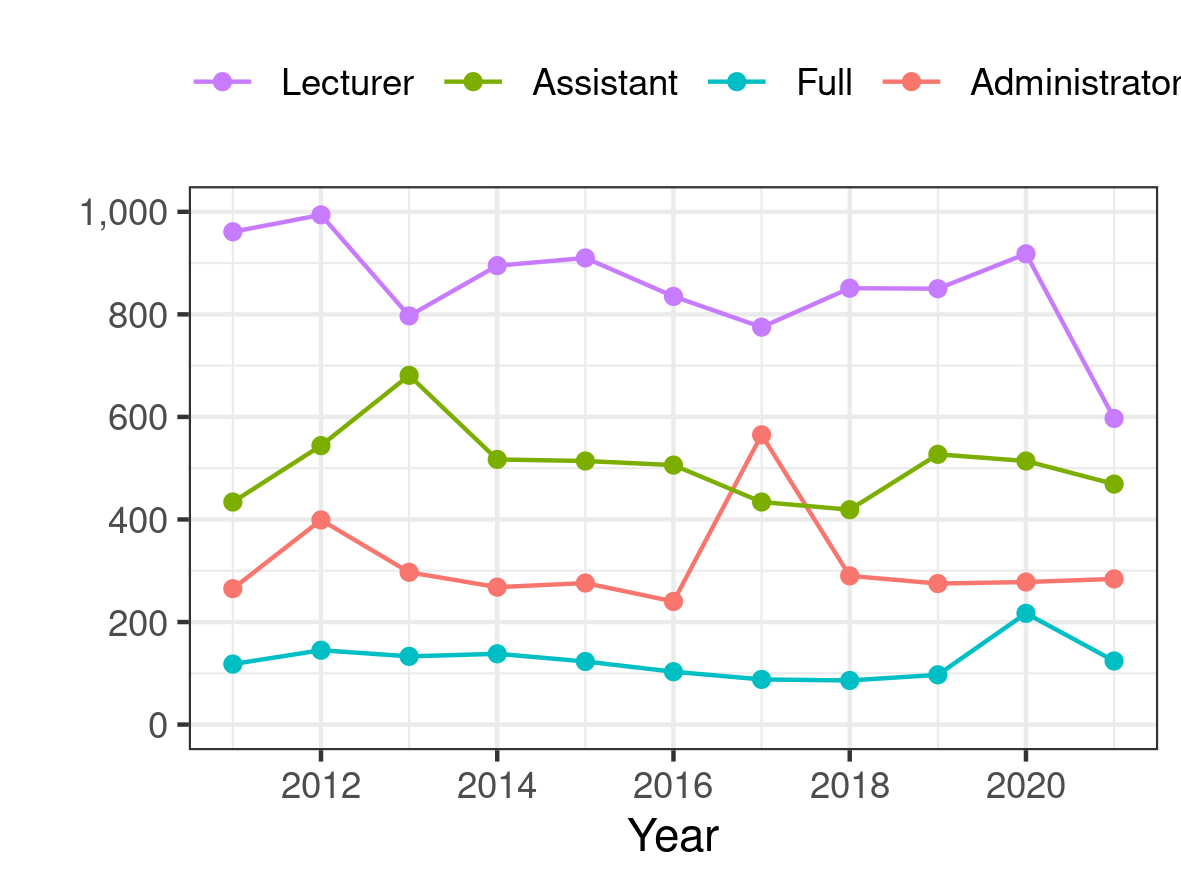
\includegraphics[width=\textwidth]{figures/newhire-count-illinois.png}
        \label{fig:newhire-count-illinois}
    \end{subfigure}
    \begin{subfigure}[b]{0.495\textwidth}
        \centering
        \caption{Mean Salary in First Year for New Hires, \$ 2021 CPI-U.}
        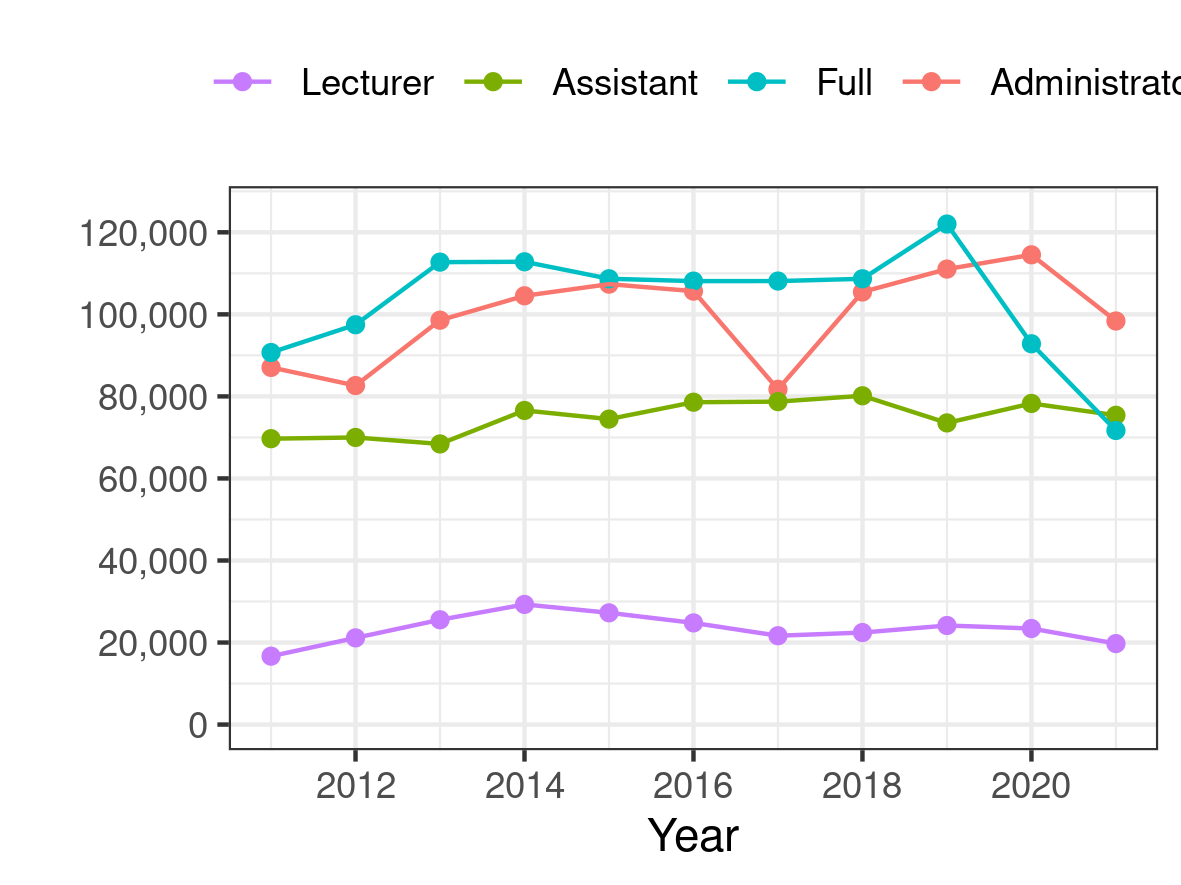
\includegraphics[width=\textwidth]{figures/newhire-salary-illinois.png}
        \label{fig:newhire-salary-illinois}
    \end{subfigure}
    \label{fig:newhire-illinois}
\end{figure}

These examples show that Illinois public universities were effected by the negative shock to state funding for higher education, and instituted policy changes aimed at affecting faculty outcomes investigated in \autoref{sec:results}.
Yet the only measurable effect was on count of professor per student (implied via slower hiring), and first-year lecturer salaries.
To investigate these trends for the entire state, \autoref{fig:newhire-illinois} shows the count of professors hired in the years 2011-2021, and their mean salary, by position.
In particular, no position had sustained rises in hiring while enrolment within the university was rising (so that new hires per student necessarily fell), and hiring of new administrators jumped once the Illinois budget crisis ended in 2017.
At the same time, professor new hires' starting salaries remained relatively constant for lecturer and assistant professors, yet rose and fell over the decade for full professors and administrators.

% Conclusion
%%%%%%%%%%%%%%%%%%%%%%%%%%%%%%%%%%%%%%%%%
%% Conclusion section
\section{Summary and Concluding Remarks}
\label{sec:conclusion}

This analysis investigates how the recent stagnation in state support for higher education has affected public universities, and their faculty composition.
The work contributes to the literature along two primary dimensions.
Firstly, by exploiting the same empirical approach as \cite{NBERw23736,NBERw27885} to isolate the causal effect of changes in state funding on public universities themselves, the analysis provides a plausible mechanism for the observed negative effects on students outcomes that this stagnation has brought.
Secondly, this analysis considers individual professors as the unit of analysis using a dataset (IBHED) new in the economic literature.
These data allow for detailed analysis of thousand's of professors' salaries, and are a starting point for further analysis of the determinants of professors wages in the Illinois public university system. 

Findings show that public universities have substituted away from tenure-track and tenured professors, towards non-tenured lecturers, in the face of persistent declines in state funding for higher education.
The effects on incumbent professors in the state of Illinois are non-distinguishable from zero, which implies that the effect is driven by changes in university hiring of new professors.
Public universities are hiring thousands of non-tenured lecturers to satisfy teaching obligations, and fewer tenure-track and tenured professors that their private counterparts.

While costs education have been rising in the US, thanks to multiple overlapping trends \citep{ehrenberg2012}, public universities have also dealt with declining state support.
It is natural to expect that such headwinds will lead to systematic change at public universities, changes which are not neutral to the composition of faculty, or to their goals of research and education.
Thes results show large changes in faculty composition, and that stagnation in state support explains at least a third of the observed shift away from tenured professors and towards contingent lecturers.
At the same time, private universities were not exposed to financial headwinds of the same magnitude or persistence.
If public universities' hiring of faculty is disrupted by a fall in state funding, then we can expect that private universities will benefit (in a competitive sense) by being able to hire better professors from relatively resource constrained public universities.
While public universities continue to educate the majority of higher education students in the US, we should worry about the effects that restricting their financial support has on the composition of faculty, and  higher education itself, in this country.


% Bibliography
\singlespacing
\bibliographystyle{agsm}
\bibliography{sections/08-bibliography.bib}
% Appendix
%%%%%%%%%%%%%%%%%%%%%%%%%%%%%%%%%%%%%%%%%
%% Appendix section
% Set-up the section.
\newpage
\appendix
\setcounter{table}{0}
\renewcommand{\thetable}{A\arabic{table}}
\setcounter{figure}{0}
\renewcommand{\thefigure}{A\arabic{figure}}

% Start appendix
\section{Appendix}
\label{appendix}
This project used data which are fully public, and computational tools which are fully open-source.
As such, all code and data involved in this project are available at this project's Github repository, available at \url{https://github.com/shoganhennessy/state-faculty-composition}.
They may be used for replication, or as the basis for further work, as needed.
Any comments or suggestions may be sent to me at \href{mailto:seh325@cornell.edu}{\nolinkurl{seh325@cornell.edu}}, or raised as an issue on the Github project.

A number of statistical packages, for the $R$ language \citep{R2022}, made the empirical analysis for this paper possible.
\begin{itemize}
    \item \textit{Tidyverse} \citep{tidyverse} collected tools for data analysis in the R language.
    \item \textit{LFE} \citep{lfe} implemented linear fixed effect models, with instruments, crucial for the empirical estimation in \autoref{sec:empirics}.
    \item \textit{Stargazer} \citep{stargazer} provided a method to efficiently convert empirical results into presentable output in \LaTeX.
    \item \textit{Lpirfs} \citep{lpirfs2019} implemented estimation of the \cite{jorda2005} local projections methods, with instrumental variables, crucial to the local projections estimates presented in this project.
\end{itemize}


\subsection{First Stage Estimates, Individual Outcomes}
\label{appendix:part1}

\begin{table}[h!]
    \singlespacing
    \centering
    \caption{IBHED Summary Statistics, Entire Professor Panel 2010--2021.}
    \makebox[\textwidth][c]{
\begin{tabular}{@{\extracolsep{5pt}}lcccc} 
\\[-1.8ex]\hline 
\hline \\[-1.8ex] 
Statistic & \multicolumn{1}{c}{Mean} & \multicolumn{1}{c}{St. Dev.} & \multicolumn{1}{c}{Median} & \multicolumn{1}{c}{N} \\ 
\hline \\[-1.8ex] 
Lecturer, percent & 38 & 48 & 0 & 68,449 \\ 
Assistant professor, percent & 32 & 47 & 0 & 68,449 \\ 
Full professor, percent & 13 & 34 & 0 & 68,449 \\ 
Administrator professor, percent & 17 & 37 & 0 & 68,449 \\ 
Lecturer salary (2021 USD) & 27,931 & 25,783 & 18,729 & 25,820 \\ 
Assistant salary (2021 USD) & 79,842 & 37,139 & 75,541 & 22,156 \\ 
Full salary (2021 USD) & 108,252 & 57,567 & 97,527 & 9,001 \\ 
Administrator salary (2021 USD) & 111,256 & 62,519 & 99,012 & 11,472 \\ 
All salary (2021 USD) & 69,261 & 54,443 & 65,954 & 68,449 \\ 
Lecturer benefits (2021 USD) & 1,930 & 6,951 & 0 & 25,820 \\ 
Assistant benefits (2021 USD) & 2,820 & 7,067 & 0 & 22,156 \\ 
Full benefits (2021 USD) & 5,892 & 13,476 & 0 & 9,001 \\ 
Administrator benefits (2021 USD) & 3,188 & 19,671 & 0 & 11,472 \\ 
All benefits (2021 USD) & 2,950 & 11,165 & 0 & 68,449 \\ 
\hline \\[-1.8ex] 
\end{tabular} 
}
    \label{tab:illinois-summary-rolling}
    \begin{flushleft}
        \footnotesize
        \textbf{Note}: This table presents the summary statistics for professors with an observed year of first-year at their university.
    \end{flushleft}
\end{table}

\begin{table}[H]
    \singlespacing
    \centering
    \caption{First Stage Estimates, for Total University Revenues at the Individual-Level.}
    \makebox[\textwidth][c]{
\begin{tabular}{@{\extracolsep{5pt}}lcccc} 
\\[-1.8ex]\hline 
\hline \\[-1.8ex] 
 & \multicolumn{4}{c}{Dependent Variable: State Funding} \\ 
\cline{2-5} 
\\[-1.8ex] & (1) & (2) & (3) & (4)\\ 
\hline \\[-1.8ex] 
 Appropriations Shock & 0.939 & 0.486 & 0.920 & 0.328 \\ 
  & (0.024) & (0.084) & (0.024) & (0.066) \\ 
  Tuition Revenue & 0.711 & 0.766 &  &  \\ 
  & (0.223) & (0.280) &  &  \\ 
  Constant &  & $-$1.906 &  & 6.484 \\ 
  &  & (2.827) &  & (0.549) \\ 
 \hline \\[-1.8ex] 
Fixed effects? & Yes & No & Yes & No \\ 
F stat. & 754.498 & 17.745 & 1470.24 & 24.842 \\ 
Observations & 68,449 & 68,449 & 68,449 & 68,449 \\ 
R$^{2}$ & 0.911 & 0.416 & 0.906 & 0.257 \\ 
\hline 
\hline \\[-1.8ex] 
\end{tabular} 
}
    \label{tab:firststage-illinois}
    \begin{flushleft}
        \footnotesize
        \textbf{Note}: Standard errors are clustered at the university-year level.
    \end{flushleft}
\end{table}


\begin{figure}[h!]
    \centering
    \singlespacing
    \caption{Local Projection Estimates for First-Stage \autoref{eqn:secondstage1_indiv}.}
    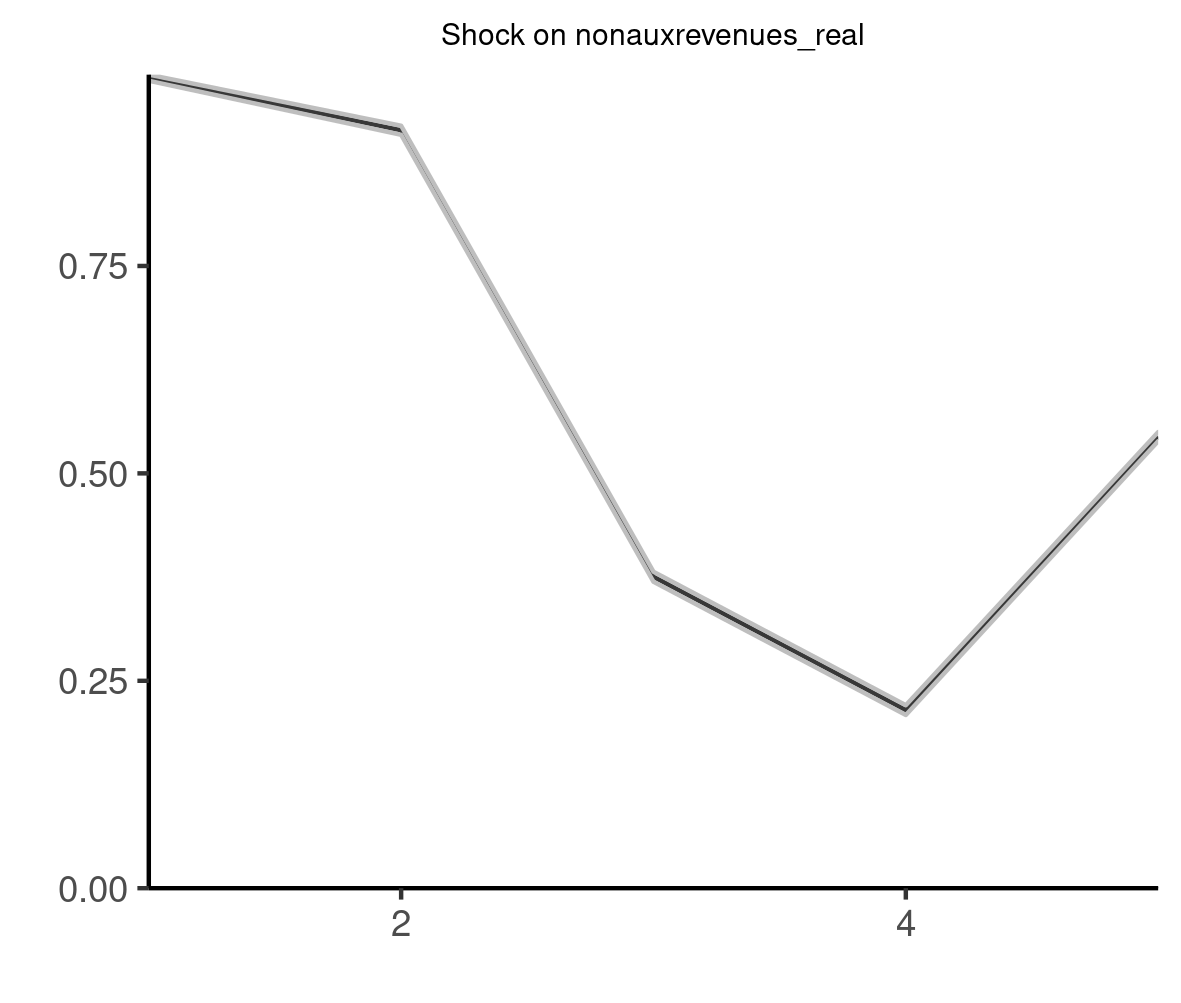
\includegraphics[width=0.6\textwidth]{figures/firststage-illinois-lp-rolling.png}
    \label{fig:firststage-illinois-lp}
\end{figure}


\subsection{Additional Results, University-Level}

\autoref{tab:facultysalaries-shock-reg} presents OLS and IV estimates where the outcome is (log) mean salary for professors employed at the university, separated by position.
Similarly, \autoref{fig:all-salaries-lp} shows the staying-power via projection methods.
The outcome, mean salary is crude.

\begin{table}[H]
    \singlespacing
    \centering
    \caption{OLS and 2SLS Estimates for University Faculty-Tenure Composition.}
    \makebox[\textwidth][c]{
\begin{tabular}{@{\extracolsep{5pt}}lcccccccc} 
\\[-1.8ex]\hline 
\hline \\[-1.8ex] 
 & \multicolumn{8}{c}{Dependent Variable: Employment Count by Tenure Group} \\ 
\cline{2-9} 
\\[-1.8ex] & \multicolumn{2}{c}{Non-tenure} & \multicolumn{2}{c}{Tenure-Track} & \multicolumn{2}{c}{Tenured} & \multicolumn{2}{c}{All} \\ 
 & OLS & 2SLS & OLS & 2SLS & OLS & 2SLS & OLS & 2SLS \\ 
\\[-1.8ex] & (1) & (2) & (3) & (4) & (5) & (6) & (7) & (8)\\ 
\hline \\[-1.8ex] 
 State Funding & $-$0.0004 & 1.499 & 0.048 & 1.926 & 0.051 & 0.267 & 0.037 & 0.893 \\ 
  & (0.016) & (10.764) & (0.051) & (8.050) & (0.029) & (1.104) & (0.023) & (4.610) \\ 
 \hline \\[-1.8ex] 
Observations & 4,825 & 4,825 & 5,094 & 5,094 & 5,130 & 5,130 & 5,181 & 5,181 \\ 
R$^{2}$ & 0.849 & 0.588 & 0.777 & $-$0.413 & 0.898 & 0.872 & 0.932 & 0.426 \\ 
\hline 
\hline \\[-1.8ex] 
\end{tabular} 
}
    \begin{flushleft}
        \footnotesize
        \textbf{Note}: Standard errors are clustered at the university-year level.
    \end{flushleft}
    \label{tab:tenurecount-shock-reg-fte}
\end{table}

\begin{table}[H]
    \singlespacing
    \centering
    \caption{OLS and 2SLS Estimates for University Faculty Salaries.}
    \makebox[\textwidth][c]{
\begin{tabular}{@{\extracolsep{5pt}}lcccccccc} 
\\[-1.8ex]\hline 
\hline \\[-1.8ex] 
 & \multicolumn{8}{c}{Dependent Variable: Mean Salary by Professor Group} \\ 
\cline{2-9} 
\\[-1.8ex] & \multicolumn{2}{c}{Lecturer} & \multicolumn{2}{c}{Assistant} & \multicolumn{2}{c}{Full} & \multicolumn{2}{c}{All} \\ 
 & OLS & 2SLS & OLS & 2SLS & OLS & 2SLS & OLS & 2SLS \\ 
\\[-1.8ex] & (1) & (2) & (3) & (4) & (5) & (6) & (7) & (8)\\ 
\hline \\[-1.8ex] 
 Appropriations Shock & 0.039 & 0.135 & 0.032 & 0.078 & 0.042 & 0.135 & $-$0.031 & 0.089 \\ 
  & (0.013) & (0.068) & (0.017) & (0.063) & (0.018) & (0.081) & (0.036) & (0.142) \\ 
  Tuition Revenue & 0.010 & $-$0.026 & 0.048 & 0.030 & 0.043 & 0.007 & 0.049 & 0.002 \\ 
  & (0.015) & (0.027) & (0.013) & (0.026) & (0.016) & (0.032) & (0.031) & (0.057) \\ 
 \hline \\[-1.8ex] 
Observations & 16,260 & 16,260 & 17,212 & 17,212 & 17,317 & 17,317 & 17,397 & 17,397 \\ 
R$^{2}$ & 0.682 & 0.678 & 0.823 & 0.822 & 0.855 & 0.851 & 0.412 & 0.411 \\ 
\hline 
\hline \\[-1.8ex] 
\end{tabular} 
}
    \begin{flushleft}
        \footnotesize
        \textbf{Note}: Standard errors are clustered at the state-year level.
    \end{flushleft}
    \label{tab:facultysalaries-shock-reg}
\end{table}

\begin{figure}[H]
    \centering
    \singlespacing
    \caption{Local Projection Estimates for Professor Salary, Mean within Each University.}
    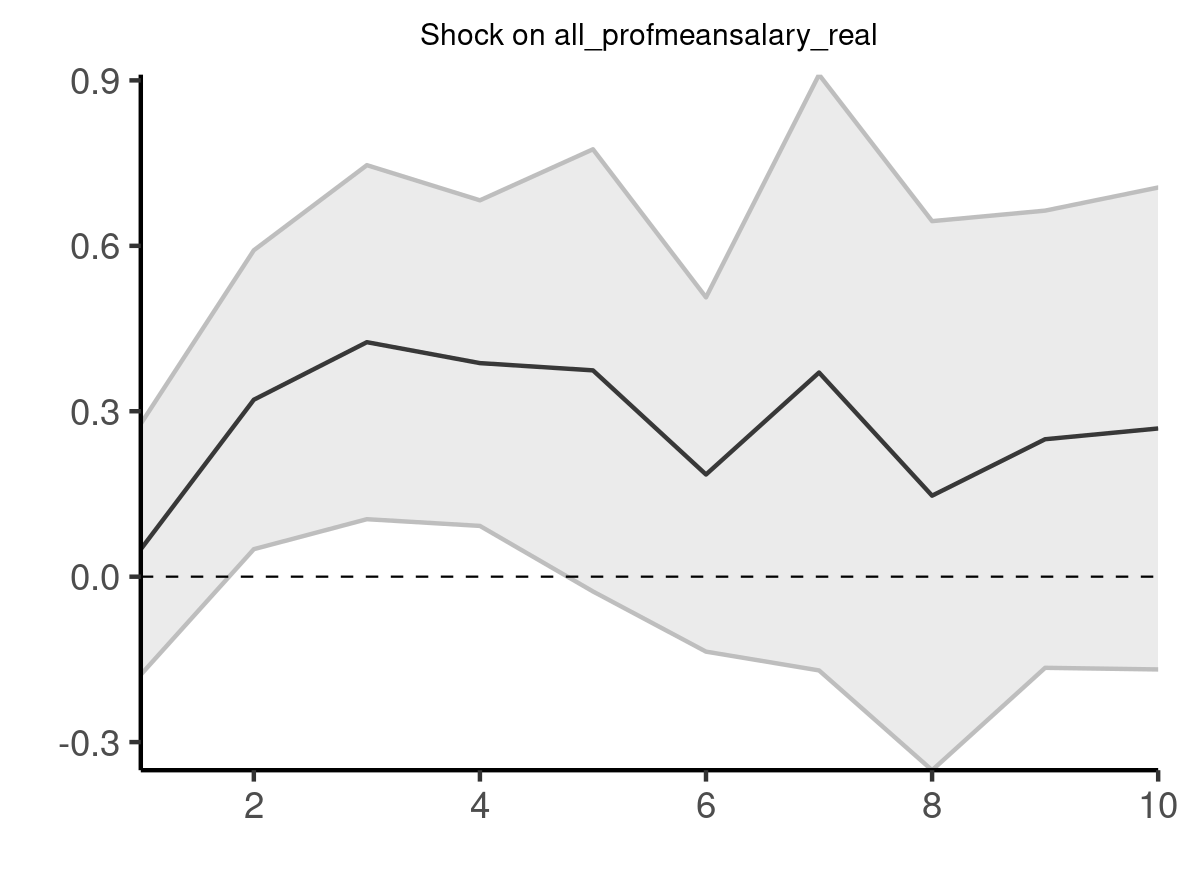
\includegraphics[width=0.6\textwidth]{figures/all-salaries-lp.png}
    \label{fig:all-salaries-lp}
\end{figure}


\subsection{Additional Results, Individual-Professor Level}

\begin{table}[H]
    \singlespacing
    \centering
    \caption{2SLS Estimates for Faculty Salaries at Illinois Universities.}
    \makebox[\textwidth][c]{
\begin{tabular}{@{\extracolsep{5pt}}lccccc} 
\\[-1.8ex]\hline 
\hline \\[-1.8ex] 
 & \multicolumn{5}{c}{Dependent Variable: Salaries by Professor Group} \\ 
\cline{2-6} 
 & Lecturer & Assistant & Full & Admin & All \\ 
\\[-1.8ex] & (1) & (2) & (3) & (4) & (5)\\ 
\hline \\[-1.8ex] 
 Non-inst. Revenues & $-$0.306 & $-$0.216 & $-$0.069 & $-$0.117 & $-$0.222 \\ 
  & (0.139) & (0.105) & (0.030) & (0.097) & (0.133) \\ 
  Tuition Revenue & 0.769 & $-$0.416 & 0.005 & 0.468 & 0.740 \\ 
  & (0.465) & (0.310) & (0.106) & (0.246) & (0.309) \\ 
 \hline \\[-1.8ex] 
Observations & 49,637 & 39,051 & 68,243 & 28,639 & 185,570 \\ 
R$^{2}$ & 0.185 & 0.064 & 0.078 & 0.130 & 0.140 \\ 
\hline 
\hline \\[-1.8ex] 
\end{tabular} 
}
    \begin{flushleft}
        \footnotesize
        \textbf{Note}: Standard errors are clustered at the institution-year level.
    \end{flushleft}
    \label{tab:facultysalaries-shock-illinois}
\end{table}

\begin{table}[H]
    \singlespacing
    \centering
    \caption{2SLS Estimates for Faculty Promotion Rate at Illinois Universities, using Rolling Instrument.}
    \makebox[\textwidth][c]{
\begin{tabular}{@{\extracolsep{5pt}}lcccc} 
\\[-1.8ex]\hline 
\hline \\[-1.8ex] 
 & \multicolumn{4}{c}{Dependent Variable: Promotion Rate by Professor Group} \\ 
\cline{2-5} 
 & Lecturer & Assistant & Associate & All \\ 
\\[-1.8ex] & (1) & (2) & (3) & (4)\\ 
\hline \\[-1.8ex] 
 Non-inst. Revenues & 0.014 & 0.035 & 0.029 & 0.014 \\ 
  & (0.007) & (0.019) & (0.062) & (0.009) \\ 
 \hline \\[-1.8ex] 
Observations & 16,346 & 17,094 & 4,377 & 42,396 \\ 
R$^{2}$ & 0.007 & 0.024 & 0.029 & 0.009 \\ 
\hline 
\hline \\[-1.8ex] 
\end{tabular} 
}
    \begin{flushleft}
        \footnotesize
        \textbf{Note}: Standard errors are clustered at the institution and first year of employment level.
    \end{flushleft}
    \label{tab:promotion-shock-illinois-rolling}
\end{table}

\begin{table}[H]
    \singlespacing
    \centering
    \caption{2SLS Estimates for Faculty Promotion Rate at Illinois Universities, using Base-Year Instrument.}
    \makebox[\textwidth][c]{
\begin{tabular}{@{\extracolsep{5pt}}lcccc} 
\\[-1.8ex]\hline 
\hline \\[-1.8ex] 
 & \multicolumn{4}{c}{Dependent Variable: Promotion Rate by Professor Group} \\ 
\cline{2-5} 
 & Lecturer & Assistant & Associate & All \\ 
\\[-1.8ex] & (1) & (2) & (3) & (4)\\ 
\hline \\[-1.8ex] 
 Non-inst. Revenues & 0.051 & 0.063 & $-$0.002 & 0.010 \\ 
  & (0.028) & (0.031) & (0.036) & (0.013) \\ 
  Tuition Revenue & $-$0.086 & $-$0.180 & $-$0.231 & 0.008 \\ 
  & (0.040) & (0.061) & (0.082) & (0.024) \\ 
 \hline \\[-1.8ex] 
Observations & 36,097 & 39,527 & 35,978 & 135,221 \\ 
R$^{2}$ & 0.014 & 0.019 & 0.027 & 0.004 \\ 
\hline 
\hline \\[-1.8ex] 
\end{tabular} 
}
    \begin{flushleft}
        \footnotesize
        \textbf{Note}: Standard errors are clustered at the institution and first year of employment level.
    \end{flushleft}
    \label{tab:promotion-shock-illinois}
\end{table}

\begin{figure}[H]
    \centering
    \singlespacing
    \caption{Local Projection Estimates for Promotion Rate at Illinois Universities.}
    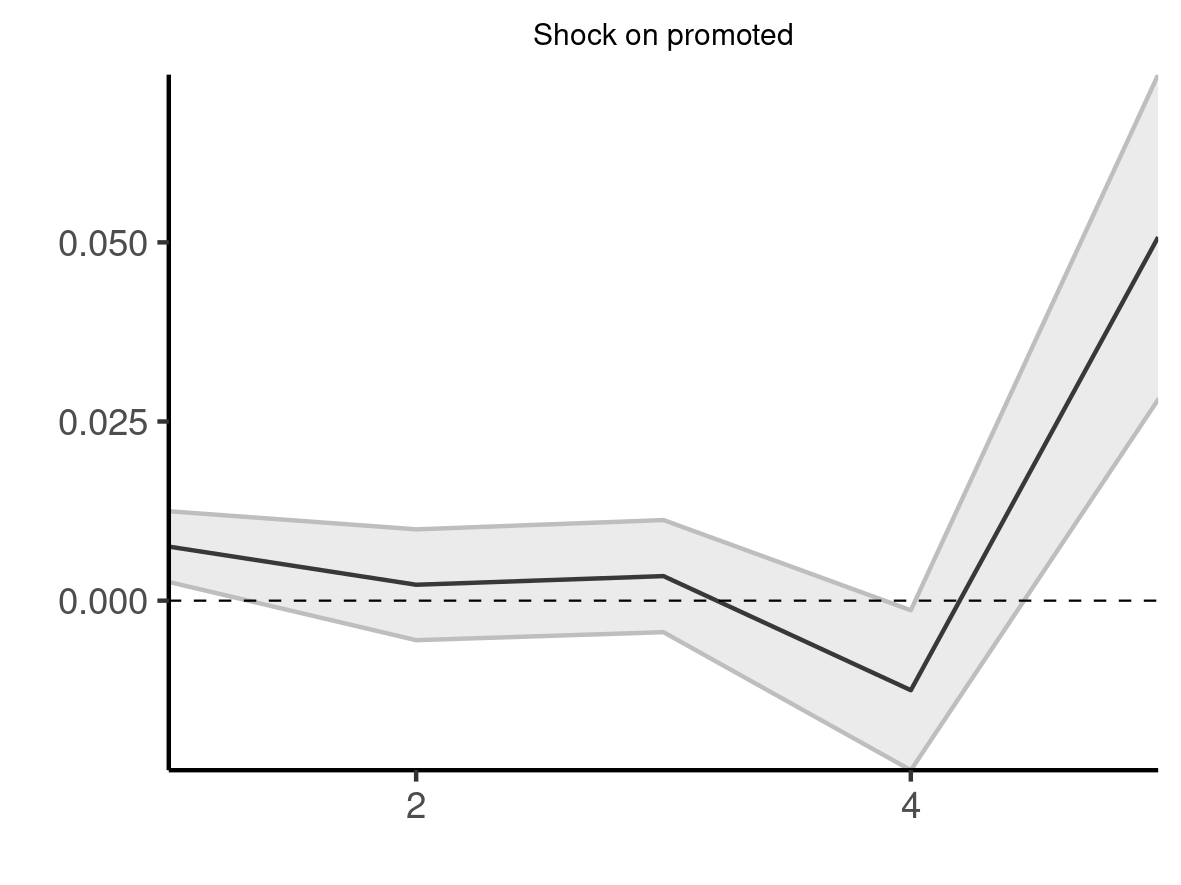
\includegraphics[width=0.6\textwidth]{figures/promoted-illinois-lp-rolling.png}
    \label{fig:promoted-illinois-lp}
\end{figure}

\begin{table}[H]
    \singlespacing
    \centering
    \caption{2SLS Estimates for Faculty Exit Rate at Illinois Universities, using Rolling Instrument.}
    \makebox[\textwidth][c]{
\begin{tabular}{@{\extracolsep{5pt}}lccccc} 
\\[-1.8ex]\hline 
\hline \\[-1.8ex] 
 & \multicolumn{5}{c}{Dependent Variable: Exit rate by Professor Group} \\ 
\cline{2-6} 
 & Lecturer & Assistant & Full & Admin & All \\ 
\\[-1.8ex] & (1) & (2) & (3) & (4) & (5)\\ 
\hline \\[-1.8ex] 
 Non-inst. Revenues & $-$0.007 & 0.002 & $-$0.004 & $-$0.003 & $-$0.006 \\ 
  & (0.024) & (0.006) & (0.008) & (0.020) & (0.015) \\ 
 \hline \\[-1.8ex] 
Observations & 23,376 & 19,757 & 7,190 & 10,191 & 60,514 \\ 
R$^{2}$ & 0.013 & 0.006 & 0.014 & 0.068 & 0.016 \\ 
\hline 
\hline \\[-1.8ex] 
\end{tabular} 
}
    \begin{flushleft}
        \footnotesize
        \textbf{Note}: Standard errors are clustered at the institution and first year of employment level.
    \end{flushleft}
    \label{tab:facultyleaving-shock-illinois-rolling}
\end{table}

\begin{table}[H]
    \singlespacing
    \centering
    \caption{2SLS Estimates for Faculty Exit Rate at Illinois Universities, using Base-Year Instrument.}
    \makebox[\textwidth][c]{
\begin{tabular}{@{\extracolsep{5pt}}lccccc} 
\\[-1.8ex]\hline 
\hline \\[-1.8ex] 
 & \multicolumn{5}{c}{Dependent Variable: Exit rate by Professor Group} \\ 
\cline{2-6} 
 & Lecturer & Assistant & Full & Admin & All \\ 
\\[-1.8ex] & (1) & (2) & (3) & (4) & (5)\\ 
\hline \\[-1.8ex] 
 Non-inst. Revenues & $-$0.009 & 0.0001 & 0.001 & 0.018 & 0.004 \\ 
  & (0.015) & (0.003) & (0.003) & (0.020) & (0.009) \\ 
 \hline \\[-1.8ex] 
Observations & 45,734 & 35,882 & 62,499 & 26,337 & 170,452 \\ 
R$^{2}$ & 0.030 & 0.005 & 0.003 & 0.026 & 0.016 \\ 
\hline 
\hline \\[-1.8ex] 
\end{tabular} 
}
    \begin{flushleft}
        \footnotesize
        \textbf{Note}: Standard errors are clustered at the institution and first year of employment level.
    \end{flushleft}
    \label{tab:facultyleaving-shock-illinois}
\end{table}
\end{document}
